\hypertarget{empirical-analysis}{%
\chapter{Empirical Analysis}\label{empirical-analysis}}

\hypertarget{introduction}{%
\section{Introduction}\label{introduction}}

The five competing explanations specified in the preceding chapters
(Chapters 2 and 3) are tested here against the documentary evidence:
capital constraints, fiscal regime effects, regulatory inadequacy,
political economy, and capability-related factors. Coordination failure
accompanies them as an observable feature of all unsuccessful cases, a
symptom the analysis tracks among the outcomes the five explanations
must account for. Support accrues to an explanation only when the
evidence matches its own pre-specified predictions; the elimination of
its rivals lies outside that standard. The presentation of evidence in
each case precedes and grounds the verdict on it, and a single
observable pattern can bear on more than one explanation at once. The
six operations proceed in order: the outcomes first, then a test of
which explanations apply, then each explanation's falsification
conditions. Then come a weighing of the survivors, then discrimination
among those that jointly survive where the evidence permits, and finally
an assessment of substitutability and externality.

The two outcome dimensions, production performance and operational
integrity, come from a descriptive account of the differentiated
outcomes (Section 4.2). The order of the analytical cases then follows
their discriminating power. The critical experiment, Aiteo on OML 29,
supplies the primary discrimination: the case where the five
explanations generate divergent predictions that the evidence can
adjudicate (Section 4.3). Eroton on OML 18 comes next as a test of
whether that pattern recurs in another operator, a partial replication
complicated by its dependence on a trunk line that Aiteo operated
(Section 4.4). First Hydrocarbon on OML 26 follows as a screening case,
since executive fraud dominates its trajectory and the case bears on the
regulatory screening gap. Three theoretical replications, Seplat on OMLs
4, 38, and 41, Shoreline and HEOSL on OML 30, and NPDC across multiple
licenses, test whether operators who differ on knowledge inheritance
produce different outcomes under comparable conditions (Section 4.5).
The marginal field program then provides a structural precedent, an
earlier and independent transfer that used government licensing in place
of a bilateral sale (Section 4.6).

Because every primary divestment case originates in the Shell divestment
wave, the cross-case synthesis also draws on three non-Shell
transactions, Oando and ConocoPhillips, Oando and Eni, and Seplat and
ExxonMobil, as seller-independence checks (Section 4.7). That synthesis
renders a verdict on each explanation and discriminates among those that
jointly survive. It then weighs the substitutability and externality
conditions that bear on the third research question, where the
Renaissance transaction offers a design contrast. The unresolved
ambiguities come last (Section 4.8).

Documentary evidence grounds the verdicts. Production figures come from
audited and regulatory records, principally NEITI annual audits and
NUPRC reports. The Wood Mackenzie Nigeria Upstream Summary (2026), a
commercial modeled series, provides a consistent panel for the five
formal case licenses, where comparable license-level series are
available, over 2016 to 2025. The two series appear together where they
overlap and stay separate where they diverge, with the reason given.
Flare intensity from NEITI audits, spill records via NOSDRA and the SDN
environmental index, corporate disclosures, statutory texts, regulatory
statements, and court records complete the evidence base, weighted by
source quality (Section 3.3). Spill records enter mainly for discrete,
undisputed events, since operator-level spill comparison is unreliable
across sources (Section 4.2). Where participant testimony was obtained,
it appears within the relevant case analysis, with documentary evidence
taking precedence.

The resulting claim matches what the design can support. Identifying
which explanation is most consistent with the observable evidence, after
every explanation has faced its own falsification conditions, is pattern
consistency under pre-specified discrimination, a standard weaker than
causal proof, and it generalizes to theoretical propositions through
analytic generalization (Yin, 2009). The evidence may point to a single
explanation, to several that are jointly necessary, or to distinctions
that stay open, in which case the ambiguity is the finding. Each
explanation receives, for each case and in a consolidated verdict across
the cases, the strongest verdict the evidence permits among the
categories specified in Chapter 2. These categories are: most consistent
with the evidence, consistent but not decisive, an enabling condition
insufficient on its own, rejected as sufficient, or rejected for
specific cases. Where a case lacks the observable implication needed to
test an explanation, that explanation carries the status not tested or
not applicable for the case.

\hypertarget{outcome-differentiation}{%
\section{Outcome Differentiation}\label{outcome-differentiation}}

The operators that acquired the divested assets fared differently; their
outcomes diverged across two dimensions, set out here before any
explanation is weighed. Production performance covers sustained output,
peak, and trajectory; operational integrity covers well-control events,
spills, flaring, and safety. The two dimensions stay separate because
they move independently: a population study of the divestment wave found
output and spills rising together (Rexer, 2025).

Absolute production figures come from the audited and regulatory record,
the NEITI annual audits and the NUPRC reports. The Wood Mackenzie
Nigeria Upstream Summary (2026), a commercial modeled series, supplies a
consistent panel for the five formal case licenses, Aiteo, Eroton,
Seplat, HEOSL, and First Hydrocarbon, over 2016 to 2025. NPDC and the
marginal fields fall outside this panel; their figures come from NEITI,
NUPRC, and Adekunle et al.~(2019). These series follow the
measurement-basis rule set out in Section 3.3: they are reported
separately, and where they diverge the audited figure governs.

Against the long national decline set out in Chapter 1, the 2 million
barrels per day target went unmet (NUPRC, 2024). At the population
level, the Stakeholder Democracy Network's 2018 index reported that
indigenous operators emitted more per barrel than the majors, subject to
the inconsistencies the index itself notes across reporting agencies
(SDN, 2020). Rexer (2025), an observational panel of 314 oilfields from
2006 to 2016 with limited ability to isolate operator-level causal
effects, associated divestment to indigenous operators with a 33 percent
rise in production and 10 percent more spills. Both are population means
the worst performers may dominate. Whether the same pairing of rising
output with rising integrity problems holds within an individual
operator, and which explanation accounts for it, is tested in the case
analysis. These figures are population context, and the case-level
evidence comes from the operators examined below.

The operator-level trajectories diverge sharply from the mid-2010s
onward, from sustained growth to post-acquisition collapse, and Table
4.1 records each operator's production figures with Figure 4.1 plotting
the modeled series against the audited points. Where the modeled and
audited series diverge, the audited record governs. Aiteo's 2024
regulatory figure reflects a June 2024 pipeline leak that shut the field
for most of the year, and the modeled 2024 and 2025 recovery for Aiteo
and Eroton runs above the audited record as a modeling artifact, marked
in Figure 4.1.

Operational-integrity indicators also vary widely across operators,
though each carries a caveat. Flaring, the share of an operator's
produced gas that was flared, ran from 49.5 percent for Aiteo and 35.2
percent for Eroton down to 11.4 percent for the Seplat joint venture in
2021. Chevron and NAOC, both with full gas-evacuation infrastructure,
stayed under 5 percent (NEITI, 2021). Gas infrastructure confounds the
comparison directly, since the OB3 pipeline serving the western fields
has been delayed since 2012, so the cross-operator figures are
indicative and carry little decisive weight. The recorded spill counts
differ across NOSDRA, NNPC, and the regulator for the same year, so any
operator-level spill comparison rests on figures that disagree. The
integrity evidence therefore rests on the discrete, undisputed events
set out in Section 1.2 and recorded in Table 4.1: three negative, the
Santa Barbara blowout, the 74 percent metering error in Aiteo's 2022
audited return against a 6.9 percent norm, and the July 2020 Benin River
Valve Station explosion; and one positive, Seplat's record of more than
11 million man-hours without a lost-time injury.

Setting the explanations aside for a moment, the six formal cases fall
into four groups, and the marginal field program forms a fifth. The
classification turns on each operator's later production as a share of
its post-acquisition peak. The operators that declined bottomed below 15
percent of peak, and the operators that held stayed above 70 percent.
Among the cases classified as sustained growth or deterioration, every
one falls either below 30 percent or above 70 percent, so the cutoffs
used here, 70 percent for sustained and 30 percent for deterioration,
sit inside an empty band. The classification holds regardless of their
exact placement. Aiteo fell to 4,900 metered in 2022, 12 percent of its
41,000 peak (700 fiscalized, after a 74 percent metering-error
deduction). Eroton's delivered output fell to near zero, about 600
fiscalized in 2022, below 2 percent of its 32,000 peak (the wellhead
crude metered near 9,000 but stranded short of the terminal). Seplat
held at 39,000 in 2025, 74 percent of its 53,000 peak, and HEOSL at
35,000, 100 percent. The comparator differs by operator because the
usable record does. The two declining operators are measured at their
2022 audited trough: Aiteo on metered output, since its fiscalized
figure is depressed by a 74 percent metering-error adjustment, and
Eroton on delivered volume, since its metered crude was stranded short
of the terminal. The two operators that held are measured at their 2025
modeled level, the only figure available for that year. Because those
cases fall outside the 30-to-70 band on any of these bases, the
classification is descriptive and insensitive to the choice among them.

Sustained growth covers Seplat and the HEOSL-operated OML 30. Growth
then deterioration covers Aiteo and Eroton, the latter a deterioration
of delivered output whose attribution is tested in Section 4.4.
Low-level survival covers First Hydrocarbon. Underperformance against
mandate covers NPDC, which set 500,000 barrels per day for 2020 and
recorded the lowest technical efficiency of any operator category at 23
percent, on a basis that differs from the OML-level production series
(Adekunle et al., 2019). Non-development covers the marginal field
cohort. The classification establishes that the outcomes are
heterogeneous, spanning sustained growth, deterioration, low-level
survival, underperformance against mandate, and non-development. The
reasons behind them come from the case analysis.

\begin{landscape}
\footnotesize
\begin{longtable}[]{@{}
  >{\RaggedRight\arraybackslash}p{(\columnwidth - 12\tabcolsep) * \real{0.1429}}
  >{\RaggedRight\arraybackslash}p{(\columnwidth - 12\tabcolsep) * \real{0.1429}}
  >{\RaggedRight\arraybackslash}p{(\columnwidth - 12\tabcolsep) * \real{0.1429}}
  >{\RaggedRight\arraybackslash}p{(\columnwidth - 12\tabcolsep) * \real{0.1429}}
  >{\RaggedRight\arraybackslash}p{(\columnwidth - 12\tabcolsep) * \real{0.1429}}
  >{\RaggedRight\arraybackslash}p{(\columnwidth - 12\tabcolsep) * \real{0.1429}}
  >{\RaggedRight\arraybackslash}p{(\columnwidth - 12\tabcolsep) * \real{0.1429}}@{}}
\caption[Post-divestment outcomes across the six formal cases]{Post-divestment outcomes across the formal cases, operators that acquired assets under broadly similar sectoral conditions but differ in transfer mechanism, operator structure, and asset history.}\\
\toprule\noalign{}
\begin{minipage}[b]{\linewidth}\RaggedRight
Operator (asset)
\end{minipage} & \begin{minipage}[b]{\linewidth}\RaggedRight
Acquired
\end{minipage} & \begin{minipage}[b]{\linewidth}\RaggedRight
Seller
\end{minipage} & \begin{minipage}[b]{\linewidth}\RaggedRight
Acquisition cost
\end{minipage} & \begin{minipage}[b]{\linewidth}\RaggedRight
Production performance outcome
\end{minipage} & \begin{minipage}[b]{\linewidth}\RaggedRight
Operational integrity outcome
\end{minipage} & \begin{minipage}[b]{\linewidth}\RaggedRight
Trajectory class
\end{minipage} \\
\midrule\noalign{}
\endfirsthead
\toprule\noalign{}
\begin{minipage}[b]{\linewidth}\RaggedRight
Operator (asset)
\end{minipage} & \begin{minipage}[b]{\linewidth}\RaggedRight
Acquired
\end{minipage} & \begin{minipage}[b]{\linewidth}\RaggedRight
Seller
\end{minipage} & \begin{minipage}[b]{\linewidth}\RaggedRight
Acquisition cost
\end{minipage} & \begin{minipage}[b]{\linewidth}\RaggedRight
Production performance outcome
\end{minipage} & \begin{minipage}[b]{\linewidth}\RaggedRight
Operational integrity outcome
\end{minipage} & \begin{minipage}[b]{\linewidth}\RaggedRight
Trajectory class
\end{minipage} \\
\midrule\noalign{}
\endhead
\bottomrule\noalign{}
\endlastfoot
Aiteo (OML 29) & 2015 & Shell & \$1.7B (OML 29 stake); \$2.562B with the
NCTL & Modeled peak \textasciitilde41 kb/\allowbreak{}d (Wood Mackenzie, 2026);
audited metered 38.2k (NEITI, 2021); 4.9k metered / 0.7k fiscalized
(2022); 7.4k annual (NUPRC 2024, mid-year shut-in). Reported corporate
peak 90k (Mar 2017), unsupported. & Santa Barbara blowout Nov 2021
(\textasciitilde200,000 bbl, 33 days, 41 communities); 74\% metering
error in 2022; flared 49.5\% of produced gas (2021) & Growth then
deterioration \\
Eroton (OML 18) & 2015 & Shell, Total, Eni & \$1.2B (45\% interest) &
Modeled peak \textasciitilde32 kb/\allowbreak{}d (Wood Mackenzie, 2026); audited
metered 19.3k (NEITI, 2021; delivered volumes far lower, the NCTL trunk
line unavailable); 9.0k metered / \textasciitilde0.6k fiscalized trough
(2022); 13.6k gross (NUPRC, 2024). Reported corporate peak 50k. & Output
stranded by evacuation failure; flared 35.2\% of produced gas (2021) &
Growth then delivered-output deterioration \\
First Hydrocarbon (OML 26, via Afren) & 2011 & Shell, Total, Eni & 45\%
interest (Shell 30\%, Total 10\%, Eni 5\%); \textasciitilde\$98M
reported, likely the Shell portion & \textasciitilde2 to
\textasciitilde15 kb/\allowbreak{}d modeled (WoodMac); audited metered 8.8k (NEITI,
2021), low base & Insufficient data to assess operational integrity.
Sponsor Afren entered administration July 2015; executives convicted of
fraud; \textasciitilde\$185M bank losses & Low-level survival \\
Seplat (OMLs 4, 38, 41) & 2010 & Shell & \$340M (45\%, from a \$610M
valuation) & Modeled peak \textasciitilde53 kb/\allowbreak{}d for the three OMLs
(Wood Mackenzie, 2026); audited metered 42.3k (NEITI, 2021);
company-wide peak 85.2k & 11M+ man-hours without a lost-time injury;
AfriSAFE Energy Company of the Year 2024; flared 11.4\% (JV,
OB3-confounded) & Sustained growth \\
Shoreline / HEOSL-operated (OML 30) & 2012 & Shell, Total, Eni & \$850M
(45\% interest) & Modeled peak \textasciitilde35 kb/\allowbreak{}d (Wood Mackenzie,
2026); audited metered \textasciitilde24k (NEITI, 2021) and
\textasciitilde30k (2022); grew from \textasciitilde4k after the 2017
operatorship change to an operator-reported peak near 67k by 2025; an
earlier 80k gross claim is set aside. & Rehabilitation of vessels,
wellheads, and compression; clear of major safety or environmental
incident in the documentary record surveyed; flaring reported only in
aggregate for OML 30 in the NEITI 2021 audit & Sustained growth \\
NPDC (multiple OMLs) & 2010 on & Shell equity via NNPC transfer & Equity
holdings, without a transaction cost & Target 500k by 2020 unmet; 23\%
technical efficiency, lowest of operator categories; production basis
differs from the OML series & Benin River Valve Station explosion July
2020, seven contractor workers killed & Underperformance against
mandate \\
\end{longtable}
\end{landscape}

Audited = NEITI metered or fiscalized and NUPRC figures; modeled = Wood
Mackenzie. Fiscalized production is production after metering losses and
theft are deducted; the Wood Mackenzie series is modeled field liquids
on a license-level basis. NUPRC figures are reported by company, so for
multi-OML operators they span assets beyond the case licenses; NEITI
2021 metered figures are by license. Acquisition costs: Items in the
source list and corporate filings.

Three further transactions inform the analysis at a lower evidentiary
weight, their data limited or non-comparable: an earlier transfer
mechanism that supplies a structural precedent, and two recent
acquisitions whose deliberate structure offers a design contrast. Table
4.2 records them.

\begin{longtable}[]{@{}
  >{\RaggedRight\arraybackslash}p{(\columnwidth - 6\tabcolsep) * \real{0.2500}}
  >{\RaggedRight\arraybackslash}p{(\columnwidth - 6\tabcolsep) * \real{0.2500}}
  >{\RaggedRight\arraybackslash}p{(\columnwidth - 6\tabcolsep) * \real{0.2500}}
  >{\RaggedRight\arraybackslash}p{(\columnwidth - 6\tabcolsep) * \real{0.2500}}@{}}
\caption[Structural precedent and design contrasts beyond the formal cases]{Structural precedent and design contrasts, weighted below the formal cases because the data are limited or non-comparable.}\\
\toprule\noalign{}
\begin{minipage}[b]{\linewidth}\RaggedRight
Item
\end{minipage} & \begin{minipage}[b]{\linewidth}\RaggedRight
Transaction
\end{minipage} & \begin{minipage}[b]{\linewidth}\RaggedRight
Role
\end{minipage} & \begin{minipage}[b]{\linewidth}\RaggedRight
Status / data
\end{minipage} \\
\midrule\noalign{}
\endfirsthead
\toprule\noalign{}
\begin{minipage}[b]{\linewidth}\RaggedRight
Item
\end{minipage} & \begin{minipage}[b]{\linewidth}\RaggedRight
Transaction
\end{minipage} & \begin{minipage}[b]{\linewidth}\RaggedRight
Role
\end{minipage} & \begin{minipage}[b]{\linewidth}\RaggedRight
Status / data
\end{minipage} \\
\midrule\noalign{}
\endhead
\bottomrule\noalign{}
\endlastfoot
Marginal field program (2003 round) & Government licensing of fields to
indigenous companies & Structural precedent (a different transfer
mechanism) & 7 of 24 producing at ten years; 17 of 30 onstream by 2022;
11 licenses revoked over the program's life; near 2\% of national
reserves; regulator judged the benefit to Nigeria minimal \\
Renaissance (SPDC onshore) & 2024 acquisition of Shell's onshore
subsidiary; \$2.4B & Design contrast (capability preservation structured
into the transaction) & 200,000+ bpd by April 2025; limited
post-transfer data \\
Seplat / MPNU & 2024 acquisition of ExxonMobil's Mobil Producing
Nigeria; \$800M; 40\% operated & Design contrast (a capable buyer
integrating from a different seller) & Months of post-transfer data;
FY2025 group production roughly doubled \\
\end{longtable}

\begin{figure}[H]
\centering
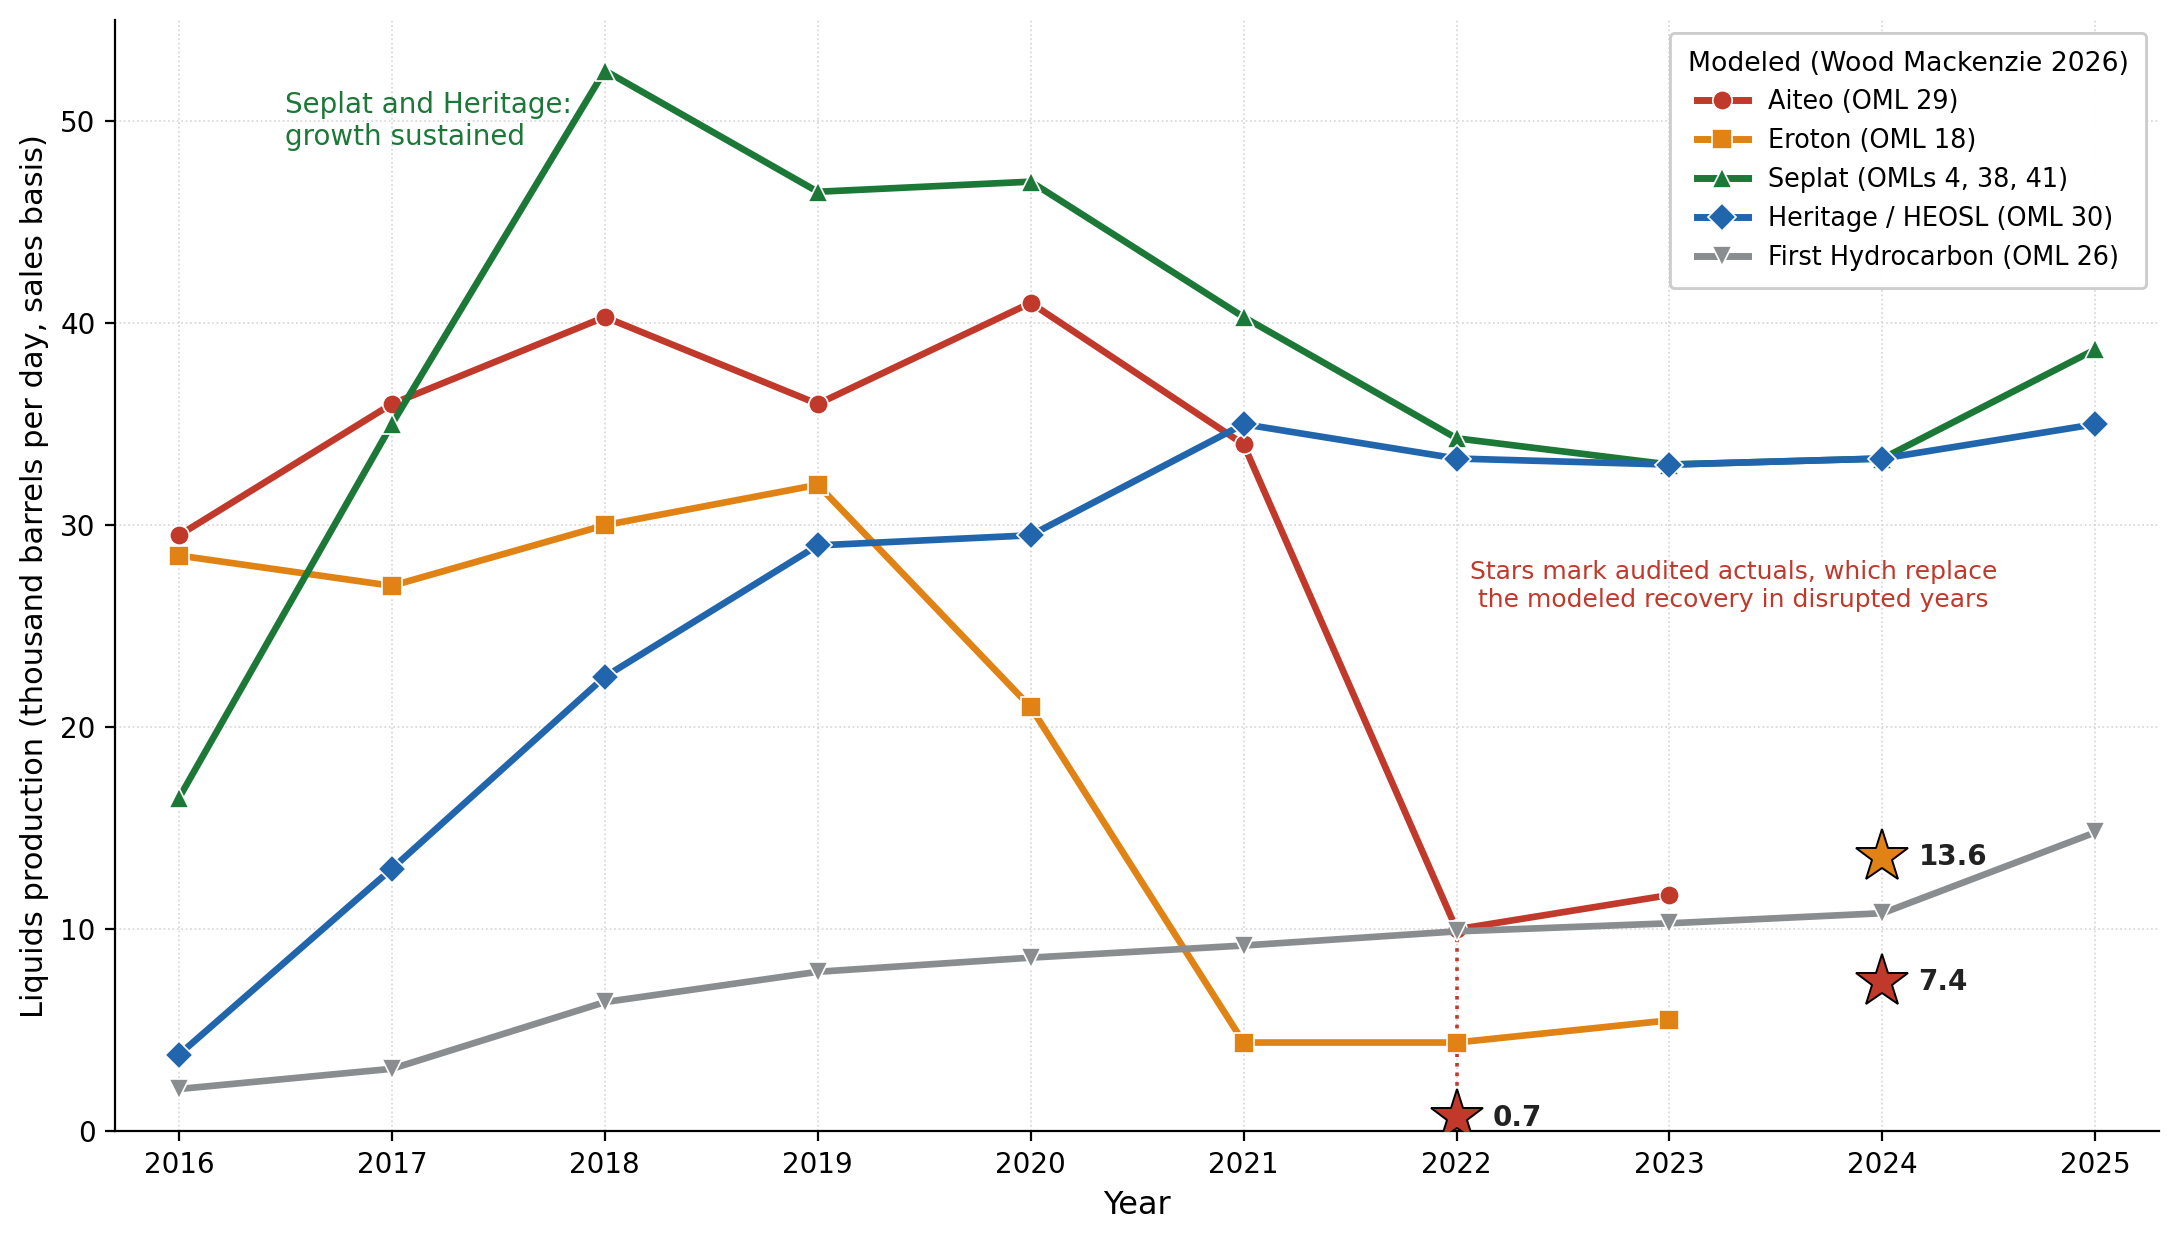
\includegraphics[width=\textwidth,height=0.45\textheight,keepaspectratio]{Figure_4_1_production_trajectories.png}
\caption[Post-divestment production trajectories of the formal case...]{Post-divestment production trajectories of the formal case OMLs. Lines show Wood Mackenzie (2026) modeled field liquids by license, on a sales basis after estimated theft; the Aiteo and Eroton lines stop at 2023, before a later modeled recovery the audited record does not support. Stars mark the audited or regulatory figures that govern in the disrupted years and fall well below the modeled lines. Where the two measurement bases diverge, the audited record governs. NPDC, the marginal cohort, and the design contrasts are omitted for want of a comparable license-level series.}
\end{figure}

\hypertarget{the-critical-experiment-aiteo-on-oml-29}{%
\section{The Critical Experiment: Aiteo on OML
29}\label{the-critical-experiment-aiteo-on-oml-29}}

Aiteo is the case where the competing explanations generate the most
divergent predictions. It is the operator that funded production growth
and then failed in a crisis beyond its capacity to contain, on an asset
acquired six years before the Petroleum Industry Act. Four of the five
explanations are tested here through their divergent predictions about
whether and how those two outcomes can co-occur in the same operator;
fiscal regime effects are eliminated separately by timing (Section
4.3.2). The documentary record adjudicates several of these differences
and bounds the rest. The positive case for capability-related factors is
built first, from the shape of the failure, before each competing
explanation is tested against its own falsification conditions; the
consolidated verdict for the case comes last (Section 4.3.6).

\hypertarget{the-selective-failure-pattern}{%
\subsection{The Selective Failure
Pattern}\label{the-selective-failure-pattern}}

Capability-related factors predict a particular shape of failure: the
knowledge-intensive parts of the operation fail while the routine parts
succeed. Routine production can often be sustained through established
procedures, contractor support, maintenance spending, and documented
operating knowledge, so an operator that inherited assets without the
embedded tacit knowledge to run them could still sustain output. The
same operator would falter when an event demanded the tacit judgment and
practiced routines that crisis response and well control require.
Aiteo's record is consistent with that shape.

On the routine side, production grew. The Wood Mackenzie modeled series
shows output on OML 29 rising over the post-acquisition years, from
about 30,000 barrels per day in 2016 to a peak near 41,000 in 2020.
Audited metered production reached 38,200 in 2021, the year before the
blowout (Wood Mackenzie, 2026; NEITI, 2021). Aiteo's announcement of a
90,000 barrel-per-day peak in March 2017 is a reported corporate figure
that sits well above the audited volumes. Part of the divergence between
reported peaks and audited volumes on the Bonny system reflects wellhead
potential measured before the pipeline-loss allocation that separates
gross from delivered crude. The gap here also exceeds what that
mechanism alone explains, and the argument holds without the figure. In
the crisis-response domain, the operation failed conspicuously. In
November 2021 the Santa Barbara Well 1 blew out and flowed uncontrolled
into the surrounding creeks until it was secured on December 8, roughly
33 days later. The joint investigation conducted by NOSDRA, the NUPRC,
the Bayelsa State Ministry of Environment, community representatives,
and well-control consultants attributed the blowout to third-party
interference. The affected community and the Bayelsa State Government
insisted that the cause was equipment failure (NOSDRA Joint
Investigation Visit, 2021; NOSDRA and NUPRC via Vanguard, 2021). The
cause is therefore contested, and the capability finding holds
independently of it. What the record establishes is a containment
failure. Aiteo assembled its well-control response after the fact,
engaging external specialists only once the blowout had occurred,
including Halliburton's Boots and Coots working with a local resource.
NOSDRA separately engaged Kenyon International for spill response, and
the well was secured only after about a month (Upstream Online, 2021;
Vanguard, 2021). The director-general of NOSDRA attributed the prolonged
failure to a capacity deficit, observing that operators forced to import
foreign well-control expertise lose critical time. He contrasted it with
the embedded arrangements an international operator carried, noting that
Shell had contained the 2011 Bonga spill quickly through a standing
worldwide spill-response subscription (NOSDRA via BusinessDay, 2021).
The investigation left the quantity spilled unsettled; independent
estimates put it near 200,000 barrels across some 41 communities, and
Aiteo disputed higher figures (NOSDRA Joint Investigation Visit, 2021;
SweetcrudeReports, 2021).

The well was a latent exposure well before it failed. Santa Barbara Well
1 had been non-producing since the 2015 acquisition; both Shell and
Aiteo left it undecommissioned, and it lay isolated, unplugged and
unmonitored, with further spills recorded in the area in 2018 and 2019.
Whether the blowout was triggered by tampering, as the official
investigation found, or by equipment failure, as the community alleged,
an idle well left in that state for six years was a standing hazard that
a fully resourced operator would have retired or kept under watch. The
capability reading turns on the containment failure that followed,
leaving the trigger aside.

Two inferences follow, and they rest on different evidence. First, the
funded production growth weakens capital constraints as the binding
explanation, in the sense of a single factor that alone accounts for the
outcome. The operator paid about \$2.562 billion for the 45 percent
interest in OML 29 and the Nembe Creek Trunk Line (HOMEF, 2021;
Nairametrics, 2015), and then funded sustained production growth
demonstrably had capital available for production-directed major
operational spending. That alone leaves open how Aiteo allocated funds
internally, so the failure turns on whether crisis readiness was
unavailable through financial scarcity or absent because the
organization had yet to put it in place. Second, and separately, the
failure points toward capability-related factors. That reading rests on
the operational evidence concentrated in the crisis-response domain,
with the funded growth bearing only on capital. That evidence is the
absence of a contingency plan, the absence of a standing well-control
contract, the dependence on contractors engaged after the fact, and the
well left undecommissioned and unmonitored. The reviewed record for the
OML 29 transaction shows no structured provision for retaining Shell
operating staff, well-control routines, or crisis-response systems.

The competing reading treats that operational evidence as a budgeting
choice: an operator with capital for production growth might simply have
declined to fund crisis readiness. The distinction matters, because a
choice to leave a known requirement unfunded is a management decision
while the absence of the readiness system altogether is a capability
gap, and both stand apart from capital constraints. The observable
evidence favors the capability reading over a pure financial-scarcity
reading. A standing well-control arrangement is a small commitment
relative to the cost of an uncontrolled blowout response, so a funds
shortage accounts poorly for its absence. The three weeks of improvised
response, in place of an executed plan, point the same way: to an
organization that had yet to institutionalize crisis readiness before
the event. Capital constraints are rejected as sufficient regardless of
which reading holds, because the funds for production growth
demonstrably existed.

The leadership's background helps make the capability reading plausible,
though on its own it leaves unproven that the gap caused the failure.
Aiteo's founder and chief executive, Benedict Peters, holds a degree in
geography and regional planning and built his career in downstream
petroleum, in trading, storage, and fuel distribution, his upstream
exploration and production experience beginning only with the
acquisition of OML 29. The downstream-only background carries less than
proof on its own; it is a mechanism-consistency indicator, since the
failure fell in the upstream well-control domain that lay outside that
experience. The operational record is the evidence that the gap operated
in practice.

\hypertarget{fiscal-regime-effects}{%
\subsection{Fiscal Regime Effects}\label{fiscal-regime-effects}}

Fiscal regime effects fail on timing. Aiteo acquired OML 29 in 2015, and
the Petroleum Industry Act was enacted on August 16, 2021, six years
later. The conditions that produced the failure were in place well
before that date: the suspended well had been left undecommissioned
since 2015, and the unremediated spills date from 2018 and 2019. A cause
must precede its effect. The blowout itself came in November 2021, three
months after the Act, but the conditions it exposed, the absent
well-control capability, the missing contingency plan, and the prior
unmanaged incidents, all predated the Act. Fiscal regime effects are
therefore rejected for this case as the primary explanation for the
observed failure.

\hypertarget{regulatory-inadequacy}{%
\subsection{Regulatory Inadequacy}\label{regulatory-inadequacy}}

The regulatory framework in force at the time of the Aiteo transaction
left operational capability outside its screen. Section 29 of the
Petroleum Act required ministerial consent to assign an Oil Mining Lease
but stopped there, leaving the buyer's ability to run the asset
untested. On the necessary-condition test, the framework indeed omitted
a capability requirement.

What the regulator did next points to a gap in the framework's content.
The rules were applied as written; what they required was too little. In
2024 the NUPRC introduced a seven-pillar divestment framework that it
described as the first of its kind in the sixty-eight-year history of
Nigerian exploration and production. Its first pillar, technical
capacity, appeared for the first time, with the Petroleum Act, internal
guidelines, and practice all silent on it before. That the NUPRC created
a capability criterion is strong evidence that the criterion was new,
and the new framework produced operational consequences beyond a
statement of intent. A divestment was initially withheld pending
assessment, and decommissioning escrow exceeding \$400 million was
secured across the 2024 transactions. Post-divestment failures
contributed to the timing of the reform, but the content of the reform,
a specific technical-capacity test new to the framework, is the mark of
a recognized design failure.

The gap's existence, on its own, sits below proof that it caused the
Aiteo failure. Causation would require that a capability gap was
identifiable at the point of transfer and non-compensable through the
market afterward. The first, identifiability at the point of transfer,
is directly supported. NOSDRA's account that containing the blowout
exceeded the operator's available capacity, the after-the-fact
engagement of external specialists, and the absent contingency plan all
concern well-control capability, which is assessable before a transfer.
An audit at the point of transaction could have tested for well-control
protocols, crisis-response arrangements, and blowout contingency
planning. The second, non-compensability through the market afterward,
is suggested by the persistence of the gap across six years of operation
and is tested across the cases that follow (Sections 4.4 and 4.7). And
the same pre-2024 regulatory framework, the Petroleum Act and DPR
oversight, governed Seplat, HEOSL, Aiteo, and NPDC; as the cases that
follow show, their outcomes diverged, so the framework permitted the
failure while leaving open which operators would fail. For the single
case, then, regulatory inadequacy is consistent with the design-gap
interpretation: an enabling condition that permitted the failure while
leaving unexplained, on its own, why Aiteo failed where others held.
Whether the absence of capability screening is necessary across the
population is a question the cross-case synthesis takes up (Section
4.7).

\hypertarget{political-economy-at-the-case-level}{%
\subsection{Political Economy at the Case
Level}\label{political-economy-at-the-case-level}}

The political-economy explanation is tested here for Aiteo specifically,
through observable case-level indicators. The population-level
association reported by Rexer (2025) supplies context, and the test here
draws on the case record. The relevant indicators are board composition,
shareholding, and any change in the theft rate on OML 29 around the
transfer. For Aiteo, the available record supports only a weak test of
those indicators: corporate registry detail on board composition and
shareholding is incomplete, and the search recovered no
operator-specific theft-rate series around the transfer. The test here
is therefore narrower, whether political access, even if present, could
explain the non-substitutable well-control failure.

The decisive consideration is where political access substitutes for
capability and where it reaches its limit. Connections can plausibly
reduce certain exposures, oil theft, or community friction managed
through elite-mediated access, the substitutable dimensions. Well
control and blowout contingency rest on experiential knowledge, and on
this non-substitutable dimension the outcome turns on what an operator
actually holds. The Aiteo record splits along exactly that line.
Whatever connections may have done for theft or community access on OML
29, preventing or containing the Santa Barbara blowout turned on
well-control capability, which only operating experience supplies.
Political economy is therefore rejected as sufficient for operational
quality on the non-substitutable dimension. It may help account for
commercial survival, since Aiteo continued operating after the blowout,
while the onset of the blowout and the operator's inability to contain
it lie outside its reach. The positive form of the test, whether
connections sustain commercial viability while operational quality stays
poor, is developed on NPDC (Section 4.5.3).

\hypertarget{coordination-failure}{%
\subsection{Coordination Failure}\label{coordination-failure}}

Coordination failure, treated throughout as an observable feature of
unsuccessful cases and a symptom of deeper causes, is tested here
against persistence and failure type. The blowout occurred in November
2021, six years after the 2015 acquisition, well beyond a short
transition period. If coordination failure were merely a transition
problem, it should appear early and ease as the operator stabilizes.
Aiteo's pattern points the other way: specific knowledge-intensive
functions failed while routine production grew, and the failure
persisted for six years. The unresolved spills of 2018 and 2019 show the
exposure persisting years before the blowout, present at year three and
still unaddressed at year six.

A failure of this duration and this shape runs counter to a coordination
problem that self-corrects through operational learning, so coordination
failure is rejected as an independent cause for this case. Its
persistence and domain-specificity are consistent instead with a
structural absence of knowledge.

\hypertarget{the-aiteo-verdict}{%
\subsection{The Aiteo Verdict}\label{the-aiteo-verdict}}

The five explanations, and the coordination feature that accompanies
them, resolve as follows for the Aiteo case. The verdicts use the
categories specified in Chapter 2 (Section 2.6), and each rests on the
explanation's own evidence, with the elimination of rivals set aside.

\begin{longtable}[]{@{}
  >{\RaggedRight\arraybackslash}p{(\columnwidth - 6\tabcolsep) * \real{0.2500}}
  >{\RaggedRight\arraybackslash}p{(\columnwidth - 6\tabcolsep) * \real{0.2500}}
  >{\RaggedRight\arraybackslash}p{(\columnwidth - 6\tabcolsep) * \real{0.2500}}
  >{\RaggedRight\arraybackslash}p{(\columnwidth - 6\tabcolsep) * \real{0.2500}}@{}}
\caption[Verdicts for the Aiteo critical experiment on OML 29]{Verdicts for the Aiteo case on OML 29, the critical experiment, where funded production growth alongside an uncontained blowout rejects the capital, fiscal, and political-economy explanations as sufficient for the integrity failure and leaves capability-related factors most consistent with the evidence.}\\
\toprule\noalign{}
\begin{minipage}[b]{\linewidth}\RaggedRight
Explanation
\end{minipage} & \begin{minipage}[b]{\linewidth}\RaggedRight
Verdict
\end{minipage} & \begin{minipage}[b]{\linewidth}\RaggedRight
Evidence anchor
\end{minipage} & \begin{minipage}[b]{\linewidth}\RaggedRight
What would change this verdict
\end{minipage} \\
\midrule\noalign{}
\endfirsthead
\toprule\noalign{}
\begin{minipage}[b]{\linewidth}\RaggedRight
Explanation
\end{minipage} & \begin{minipage}[b]{\linewidth}\RaggedRight
Verdict
\end{minipage} & \begin{minipage}[b]{\linewidth}\RaggedRight
Evidence anchor
\end{minipage} & \begin{minipage}[b]{\linewidth}\RaggedRight
What would change this verdict
\end{minipage} \\
\midrule\noalign{}
\endhead
\bottomrule\noalign{}
\endlastfoot
Capital constraints & Rejected as sufficient & \textasciitilde\$2.562B
acquisition, 45\% interest plus the Nembe Creek Trunk Line (HOMEF, 2021;
Nairametrics, 2015); audited metered growth to 38.2 kb/d (2021)
alongside the crisis failure, modeled peak near 41 kb/d; capital
demonstrably available for production-directed major operational
spending & Evidence that crisis-readiness funding was cut for financial
reasons \\
Fiscal regime effects & Rejected for this case & Transaction closed
2015; PIA enacted August 2021; the capability gap predates the Act &
None; the timing is arithmetic \\
Regulatory inadequacy & An enabling condition insufficient on its own;
system-level role tested in the cross-case synthesis (4.7) & Section 29
lacked capability criteria; the NUPRC created them in 2024; the same
pre-2024 framework produced different outcomes across operators,
developed in the cases that follow & Evidence that the framework
screened for capability and that Aiteo passed \\
Political economy & Rejected as sufficient for operational quality
(non-substitutable dimension) & Preventing or containing the blowout
required well-control capability beyond the reach of connections &
Evidence that political interference directly caused the operational
failure, beyond enabling commercial survival \\
Coordination failure & Rejected as independently caused; an observable
feature of the unsuccessful cases & Persistence at six years;
domain-specific failure; unremediated prior incidents & Evidence of a
specific coordination breakdown independent of knowledge absence \\
Capability-related factors & Most consistent with the evidence for this
case & Selective failure signature; containment failure lasting about a
month, which NOSDRA attributed to a capacity deficit; after-the-fact
reliance on external well-control specialists against absent embedded
crisis-response arrangements; six-year persistence; the documents
reviewed silent on any structured knowledge-transfer provision in the
transaction & An operator without inherited upstream knowledge handling
a comparable crisis successfully \\
\end{longtable}

Across the two outcome dimensions, the diagnostic split is clean for the
period the critical experiment turns on. In the years before the
blowout, commercial production grew while crisis-readiness stayed
absent, and the explanation most consistent with that split is one that
bears on integrity, with funding set aside, since binding capital
constraints would have suppressed production too. Output then fell
sharply after the blowout, to about 4,900 barrels per day metered in
2022, 700 fiscalized (NEITI, 2022), so the capability failure spread to
both dimensions; that loss came after the blowout, so the
capital-constraints explanation stays closed. In the terms of Chapter 2
(Section 2.2), this is a failure of the asset as a sociotechnical
system. The transaction moved the wells but not the operating
organization that had run them, and when the well reached a crisis the
well-control capability, the standing contracts, and the practiced
crisis response that the operating organization carried were not present
to contain it. This verdict reflects pattern consistency for a single
case.

Appendix E reproduces this verdict matrix for every case, recording the
evidence, confidence level, and falsification condition behind each
verdict; the analyses that follow state their verdicts in prose and
refer to that appendix for the full matrices.

\hypertarget{cross-case-validation-failure-replication-and-regulatory-screening}{%
\section{Cross-Case Validation: Failure Replication and Regulatory
Screening}\label{cross-case-validation-failure-replication-and-regulatory-screening}}

The Aiteo verdict rests on a single case. Two further operators test
whether it holds. Eroton acquired OML 18 from the same seller in the
same divestment round and, like Aiteo, grew production before losing it,
which makes it a replication candidate. Its collapse, however, ran
partly through a shared export line whose chronic, theft-driven downtime
lay largely outside Eroton's control, so the case is a partial
replication, complicated by the shared line (Section 4.4.1). First
Hydrocarbon acquired OML 26 through a buyer whose executives were later
convicted of fraud, which interrupts any reading of its operational
capability but bears directly on whether the approval process screened
buyers at all (Section 4.4.2).

\hypertarget{eroton-on-oml-18-a-partial-replication-complicated-by-a-shared-trunk-line}{%
\subsection{Eroton on OML 18: A Partial Replication Complicated by a
Shared Trunk
Line}\label{eroton-on-oml-18-a-partial-replication-complicated-by-a-shared-trunk-line}}

Eroton's early trajectory mirrored Aiteo's: acquisition from the same
2015 Shell divestment, rapid production growth, and a later collapse. A
consortium led by Midwestern Oil and Gas, with the Canadian-listed Mart
Resources and Suntrust Oil and Gas, acquired a 45 percent interest in
OML 18 from Shell, Total, and Eni in March 2015 for about \$1.2 billion.
NNPC held the remaining 55 percent, and Eroton was the designated
operator (Mart Resources, 2015; Templars, 2015). Production then grew
from a low base, and two independent sources agree on its scale and
trajectory once measurement basis is held constant. Wood Mackenzie's
modeled series puts the field near 32,000 barrels per day at its 2019
peak. The operator's own disclosures, released through its listed
financier San Leon, report full-field gross output before pipeline
losses of roughly 39,000 to 45,000 barrels per day across 2017 to 2019,
about 50,000 on a producing-day basis. Delivered sales after downtime
and allocated losses came to roughly 26,000 to 31,000 (Wood Mackenzie,
2026; San Leon Energy, 2017; 2019; 2020). The spread between these
figures follows from the measurement bases: the difference between
wellhead potential, annual gross, and the volume that survived a
pipeline-loss wedge running between 26 and 35 percent in these years.
The crude-reconciliation mechanism Wood Mackenzie documents for the
entire Bonny system and that Eroton addressed by installing
custody-transfer metering in 2018 (San Leon Energy, 2019; Wood
Mackenzie, 2026). On production and technical cost, Eroton looked
competent for several years, and NNPC recognized it as one of two
operators with the lowest technical cost per barrel (Wood Mackenzie,
2026). That initial competence separates Eroton from Aiteo, where the
well-integrity exposure later implicated in the blowout existed from
acquisition, and it is the first reason to treat Eroton as a partial
replication, short of a literal one.

The composition of the acquiring consortium is a secondary,
mechanism-consistency indicator, set out here because the verdict that
follows relies on it. Financial and business-development principals
assembled Eroton, in place of former international-oil-company
operators. Its lead figure, Onajite Okoloko of Midwestern Oil and Gas,
holds a degree in economics and a Harvard management qualification and
built his career in corporate finance and oilfield services. He was
managing director of Oando Energy Services, then in a marginal field
through Midwestern and in fertilizers through Notore, his career falling
outside well engineering and reservoir management (Africa Oil \& Gas
Report, 2013; 2015). The contrast with Seplat guards against an easy
objection. Okoloko had operated a marginal field, Midwestern's Umusadege
at about 13,000 barrels per day, just as Seplat's Austin Avuru had run
Platform Petroleum, so marginal-field experience was common to both.
What differed was that Avuru carried three decades of hands-on petroleum
engineering and reservoir management that scale to a complex asset,
where a business-development background scales less readily.
Marginal-field success was a necessary condition for a major lease, one
step on a longer path. The consortium that took OML 18 held the
financial and commercial capability to fund and acquire the asset, while
the inherited upstream operating depth to improvise under stress lay
beyond it. The background falls below proof that this gap caused the
failure; the internal record does that work.

Then delivered output fell to almost nothing. Export volumes collapsed
through 2020 and 2021, and by the time NNPC removed Eroton as operator
in March 2023 the asset had delivered near-zero export volumes for
roughly two years (NNPC via BusinessDay, 2023). The NEITI-audited figure
for 2021 had already fallen to about 19,300 barrels per day. Wood
Mackenzie's throughput record for the Bonny system shows the OML 18
evacuation fields, Cawthorne Channel and the OML 18 portion of Awoba
among them, dropping to zero from 2021, which corroborates the delivery
collapse from a source independent of the operator (NEITI, 2021; Wood
Mackenzie, 2026). The 2022 audit makes the split explicit: OML 18
metered about 9,000 barrels per day at the flow station but fiscalized
only 600 after a terminal adjustment of 1.6 million barrels, the
wellhead-to-delivered gap that defines evacuation stranding (NEITI,
2022). The collapse ran through two distinct pathways, and separating
them is the work of this case.

The first pathway is external, and it lay largely outside Eroton's
control. The Nembe Creek Trunk Line, the export route for OML 18 crude,
went into force majeure from the fourth quarter of 2021, and every
operator that depended on it went without deliveries (San Leon Energy,
2022; 2023). The line's unavailability extended well beyond that
quarter. Wood Mackenzie records the Nembe Creek Trunk Line as frequently
targeted by vandals and militant groups, with downtime that can reach 60
percent, and notes that the \$1.1 billion line Shell rebuilt in 2010
specifically to deter theft proved similarly ineffective against it.
Terminal force majeure on the Bonny system, the same source observes,
follows generically from vandalism or sabotage against the trunk
pipelines, a system-wide hazard that falls on every operator on the line
alike (Wood Mackenzie, 2026). The vulnerability was therefore structural
to the asset and the region, it predated Eroton and Aiteo alike, and it
transferred with the hardware from Shell, which had itself repeatedly
shut the line to remove theft points. Eroton kept producing at the
wellhead through the force majeure, reporting on its own account about
500,000 barrels in November 2021, an interested-source figure of roughly
16,700 barrels per day for the month. The crude meanwhile stayed short
of the Bonny terminal (San Leon Energy, 2023). The gap between metered
wellhead volume and delivered volume is the signature of evacuation
stranding: the crude is produced and metered, then held before it can be
delivered.

The line that stranded Eroton's crude was operated by Aiteo on OML 29, a
link of shared exposure to the same line. The official joint
investigation into the contemporaneous Santa Barbara incident attributed
it to third-party interference (Section 4.3), and the trunk-line force
majeures recur on the same third-party-sabotage pattern across operators
and across the periods before and after Aiteo took the line. The
available record leaves any Aiteo maintenance or surveillance failure on
the line inseparable from the regional theft and sabotage that afflict
it. The evacuation shock therefore reads best as the common environment
that every Bonny-system operator faced, a feature of the asset more than
of either operator's capability. A community suit now before the Federal
High Court alleges that Aiteo's trunk-line spills reflected operational
negligence and a failure to replace corroded pipelines, which, if
established, would reopen that reading. As of this writing the suit is
pending, with a finding yet to be made (Opu Nembe Kingdom v Aiteo,
FHC/YN/CS/284/2024).

The second pathway is internal and concerns whether Eroton could mount
an organizational response to that shock. The Federal Inland Revenue
Service sealed the company's head office for more than twelve months
over unpaid taxes; the EFCC and NUPRC opened investigations; and an NNPC
forensic audit identified governance failures (NNPC via BusinessDay,
2023; NNPC via Leadership, 2023). Most directly, an alternative barge
evacuation route won approval, and Eroton left it unexecuted, so the
crude beyond the trunk line's reach stayed stranded under the sanctioned
workaround as well (San Leon via Energy Voice, 2019, 2022a, 2022b).
These are organizational-performance failures, and they fall in the part
of the operation that Chapter 2 treats as organizational capability:
managing a regulator, sustaining joint-venture governance, and executing
a complex logistics alternative under stress are capability tasks, the
organizational work that sits above the wellhead. They are consistent
with an organizational-capability gap. The documentary record alone,
however, leaves that reading entangled with governance, liquidity, or
political dynamics, and participant testimony is the evidence that would
distinguish them.

The two pathways resist clean separation, and the case is weaker for it.
The external shock alone could have stranded a capable operator; the
internal failures alone could have sunk production even with the trunk
line intact. In the event both occurred together, and the documentary
record can only partly apportion how much of the two-year collapse each
contributed. That is the honest limit of the case, and it is why Eroton
corroborates the Aiteo pattern while leaving it unconfirmed.

Within that limit, the explanation tests run as follows. Capital
constraints are rejected as sufficient. The growth to a modeled 32,000
barrels per day, corroborated by the operator's reported gross output,
demonstrates that capital was available for production-directed major
operational spending. An operator that funded that growth held the funds
to run the asset (Wood Mackenzie, 2026; San Leon Energy, 2019). NNPC
separately stated that the joint-venture partners met their funding
obligations through the decline. That statement carries a caveat,
because NNPC made it while removing Eroton as operator, a context in
which it had an interest in placing the failure on the operator over
joint-venture underfunding. The inference against capital constraints
therefore rests more securely on the documented production growth than
on the statement. The unpaid-tax evidence may indicate liquidity stress
or governance failure, though on its own it leaves open whether the
joint venture held the capital to sustain production or to execute the
evacuation alternatives, so the verdict stands. Eroton's own rebuttal
accepted that funding was maintained; it attributed the collapse to the
trunk-line force majeure (Eroton via Petroleum Africa, 2023). Fiscal
regime effects are rejected for this case. The production deterioration
began before the Petroleum Industry Act, and the acquisition,
capability, and evacuation-dependence conditions that produced it were
all established under the pre-Act regime. The Act, enacted in August
2021, postdates the conditions that produced the collapse and stays
outside the primary explanation, even though the removal of the operator
ran into 2023. The regulatory framework in force at the 2015 acquisition
left operational and organizational capability outside its screen, the
same design gap documented for Aiteo. It permitted Eroton's acquisition
while, applying alike to every operator, leaving unexplained why Eroton
specifically collapsed, and it functions here as an enabling condition
shared across operators, short of a differentiating cause. Coordination
failure is rejected as independently caused: the collapse came six to
eight years after acquisition, well beyond a short transition period,
and a transition problem should appear early and ease as the operator
settles. Here, by contrast, the operator demonstrated routine
operational competence for several years before the collapse.

The political-economy and capability readings are harder to separate
here than at Aiteo, and the evidence is thinner. Corporate registry
detail on Eroton's board composition and shareholding is incomplete, so
the question is carried by the non-substitutability logic, the registry
record being too incomplete for a direct case-level test. Political
economy remains live for the case as a whole; it could plausibly bear on
the unpaid taxes, the regulatory treatment, or access to approvals. It
is rejected only as a sufficient explanation for the
operational-capability tasks at issue, in particular executing the
approved barge alternative, which lay beyond political access. The
capability reading is consistent with the internal pathway but not
decisive for the case, because the external trunk-line shock confounds
the attribution. The consortium's business-development composition,
established above, supports the reading only as a secondary indicator:
it is consistent with an organization that ran routine production well
while struggling to improvise an operational response under stress. The
background indicates the gap without establishing it as the cause; the
operational record in each case establishes the link.

Eroton therefore replicates the Aiteo pattern in part. An operator
without inherited upstream technical depth grew routine production and
then faltered when conditions deteriorated, which matches the Aiteo
trajectory. The collapse, however, mixed an external evacuation shock
with internal governance failure, and the evidence attributes it to
capability with less confidence than the Aiteo case permits. The verdict
reflects that ambiguity.

Appendix E records the full verdict matrix for the case, with the
evidence and the falsification condition behind each verdict.

The case adds two findings without amounting to a second proof. It
rejects capital constraints and fiscal timing on the same logic as
Aiteo, and it shows the funded-growth-then-failure pattern recurring in
a second operator assembled without inherited upstream depth. The
evacuation shock that might have supplied a second, independent line of
evidence instead confounds the capability attribution: it ran through
the trunk line as the common environment every Bonny-system operator
faced, structurally theft-driven and inherited from the seller. Whether
the pattern holds where the conditions differ on knowledge inheritance
is what the theoretical replications test, against operators facing the
same evacuation environment (Section 4.5).

\hypertarget{first-hydrocarbon-on-oml-26-a-test-of-regulatory-screening}{%
\subsection{First Hydrocarbon on OML 26: A Test of Regulatory
Screening}\label{first-hydrocarbon-on-oml-26-a-test-of-regulatory-screening}}

First Hydrocarbon Nigeria acquired a 45 percent interest in OML 26, in
the western Niger Delta, from the Shell joint venture in 2011,
completing an agreement struck in October 2010. The interest combined
the holdings of Shell at 30 percent, Total at 10 percent, and Eni at 5
percent, with the state company NPDC holding the remaining 55 percent
(First Hydrocarbon Nigeria, 2011; Wood Mackenzie, 2026). Two features
set the case apart from Aiteo and Eroton. First Hydrocarbon Nigeria was
a special-purpose vehicle created by the London-listed Afren plc to hold
Nigerian upstream assets, and Afren held 45 percent of it at completion,
rising to 70 percent by the time the company failed (Upstream Nigeria,
2018). And First Hydrocarbon Nigeria never operated OML 26: NPDC
asserted operatorship under a first-refusal clause in the joint
operating agreement and ran the asset throughout, with a joint
asset-management team formed only in 2016 (Africa Oil and Gas Report,
2012; Acha et al., 2019). The buyer was a non-operating financial
partner whose sponsor collapsed through fraud, a corporate failure that
played out entirely away from the asset's operations. For both reasons
the case lies outside a test of the buyer's operational capability, and
it enters here as a screening case. What it tests is whether the
approval framework assessed buyer fitness, and it provides the cleanest
rejection of capital constraints in the case set.

The screening question turns on the statute, and the statute is
explicit. Section 29 of the Petroleum Act required ministerial consent
to assign the lease while leaving the acquirer's fitness, capability,
and governance untested, the same statutory void documented for the
Aiteo transfer (Section 4.3.3). The buyer commanded ample capital and
corporate standing: Afren was a FTSE 250 company that peaked near \$2.6
billion in market value. First Hydrocarbon Nigeria funded the
acquisition and its initial development share through \$280 million of
facilities (First Hydrocarbon Nigeria, 2011; UK Serious Fraud Office,
2018). The acquiring entity's gap lay in corporate governance integrity,
a dimension that the approval framework reviewed here left outside any
party's remit, at approval and through any ongoing post-transfer fitness
test. Within four years of completion, Afren had collapsed into
administration, in July 2015. Its two most senior executives, the chief
executive Osman Shahenshah and the chief operating officer Shahid Ullah,
were convicted in 2018 of fraud and money laundering for a scheme they
ran while leading the company. They diverted roughly \$45 million from a
\$300 million transaction with another Nigerian partner into a Caribbean
or Bermudan shell company they controlled (UK Serious Fraud Office,
2018). The convictions stood when the Court of Appeal refused permission
to appeal in 2019, and a confiscation order of £5.45 million followed in
2020 (Court of Appeal, 2019; Energy Voice, 2020). The case leaves open
whether a Nigerian regulator would necessarily have discovered the fraud
in 2010 or 2011; it shows that the approval framework lacked any
explicit buyer-fitness or governance-integrity screen capable of making
that question part of the approval decision. The cost of the collapse
reached beyond Afren's shareholders: Nigerian banks that had lent into
the structure lost an estimated \$185 million when the company failed
(Vanguard, 2015).

Capital constraints are rejected as sufficient. The binding-constraint
version of the capital explanation requires that a shortage of funds
prevented the acquirer or the venture from running or developing the
asset. Here the acquirer commanded the resources of a
multi-billion-dollar listed company and dedicated financing facilities,
and the venture failed regardless, through a governance fraud that stood
apart from funding scarcity. Capital abundance left both the failure and
the asset's performance untouched.

Appendix E records the case's verdicts, including the dimensions it
leaves not tested, with the evidence and the falsification condition for
each.

Because NPDC operated OML 26, the asset's production reflects the state
operator's performance, the buyer's role aside. The modeled and audited
records agree that OML 26 produced only two to three thousand barrels
per day through the mid-2010s and reached roughly eight to ten thousand
around 2020 to 2021. The audited record then shows output slipping back,
well below the asset's developed capacity throughout (Wood Mackenzie,
2026; NEITI, 2020, 2022). That trajectory bears on NPDC's operatorship,
taken up in Section 4.5.3, with the buyer's inherited capability set
aside.

The case adds a dimension that neither Aiteo nor Eroton supplies. At
Aiteo the screening gap permitted an operator that proved unable to
contain a crisis. Here the same statutory gap permitted an acquirer
whose leadership was later convicted of serious fraud committed while
running the company, on an asset where the buyer never took operational
control. The two cases together show that the pre-2024 framework left
acquirers unscreened for both operational capability and governance
integrity, the void the NUPRC moved to close in 2024 (Section 4.3.3).
And the case rejects capital constraints in their starkest form, since
here the buyer held every financial advantage and failed anyway. Whether
the capability pattern that the critical experiment identified holds
where a capable operator inherits and runs the asset is the question the
theoretical replications take up next (Section 4.5).

\hypertarget{theoretical-replication-operators-that-differed-on-capability}{%
\section{Theoretical Replication: Operators That Differed on
Capability}\label{theoretical-replication-operators-that-differed-on-capability}}

The critical experiment identified a capability-related failure at
Aiteo, and the partial replication at Eroton showed a similar
funded-growth-then-collapse pattern, though there the attribution was
confounded by an external evacuation failure the documentary record
leaves entangled with internal governance (Section 4.4.1). Literal
replication predicts the same outcome where the same condition holds;
theoretical replication predicts a contrasting outcome where the
condition differs, and for a reason the theory names (Yin, 2009). The
three cases here differ from Aiteo and Eroton on capability. Seplat
acquired its leases with an experienced founding team and a technical
partner, and the capability account predicts sustained production and
integrity (Section 4.5.1). OML 30 supplies a within-asset comparison in
which the asset, owners, regulatory regime, and fiscal terms held
constant while operatorship passed from the state company to an
indigenous operator with technical capability, which isolates operator
capability more sharply than any cross-operator comparison can (Section
4.5.2). NPDC operated its acreage as a state company and underperformed
while surviving commercially, which tests political economy in the
positive form left open earlier (Section 4.5.3). All three operated
under the same pre-2024 regulatory regime as the failure cases, NPDC as
a state entity under, if anything, weaker external discipline, so the
contrast among them also tests whether regulatory inadequacy, common to
every operator, can account for outcomes that diverge.

\hypertarget{seplat-on-omls-4-38-and-41-a-founding-teams-technical-depth}{%
\subsection{Seplat on OMLs 4, 38, and 41: A Founding Team's Technical
Depth}\label{seplat-on-omls-4-38-and-41-a-founding-teams-technical-depth}}

Seplat entered upstream operations with the technical depth the failure
cases lacked, and it sustained both production and operational
integrity, the outcome the capability account predicts for a capable
operator. The case is the first theoretical replication.

Seplat Petroleum Development Company acquired a 45 percent interest in
OMLs 4, 38, and 41 from the Shell joint venture in 2010 for about \$340
million (Seplat, 2014). The depth originated with the buyer. The
reviewed record for the 2010 transaction shows no structured
capability-transfer provisions, and the knowledge that ran the assets
came from the founding team's own prior careers. Austin Avuru, the
founding chief executive, had spent more than three decades in Nigerian
petroleum engineering and reservoir management, beginning at NNPC as a
wellsite geologist and reservoir engineer and later running the
marginal-field operator Platform Petroleum. Basil Omiyi, who had led
Shell's Nigerian operations, joined the board after the founding
(Seplat, 2014). Where Eroton's principals brought a business-development
background, Seplat's brought operating depth, and the company paired it
with a technical partnership with Maurel et Prom, an established
international operator (Seplat, 2014). The founding team and the
partnership together gave Seplat the absorptive capacity to run the
assets, the buyer-side condition specified in Chapter 2; capability was
present at the buyer from the start, brought by the founding team
itself.

Production grew and held. The Wood Mackenzie modeled series puts the
three leases near a combined 53,000 barrels per day at their 2018 peak,
and the audited record shows metered production of 42,300 in 2021 and
43,100 in 2020. The modeled series holds the leases near 39,000 in 2025,
about 74 percent of peak and inside the sustained band (Wood Mackenzie,
2026; NEITI, 2020, 2021). Where Aiteo and Eroton fell to small fractions
of their post-acquisition peaks (Section 4.2), Seplat held above 70
percent of its own.

The available integrity indicators point in the same direction, though
they rest on different measurement bases. Seplat reported more than 11
million man-hours without a lost-time injury and was named AfriSAFE
Energy Company of the Year in 2024, and its joint-venture flaring ran
below the indigenous-operator figures in the 2021 audit (NEITI, 2021;
Seplat Energy, 2024). The flaring comparison is confounded by
gas-evacuation infrastructure and carries little decisive weight, and
the award is a form of recognition, carrying less evidentiary weight
than the audited regulatory data, so the indicators support the reading
jointly, as a set. Set against Aiteo's uncontrolled blowout and the
weaker integrity indicators in the failure cases, Seplat's safety record
points in the expected direction and is consistent with the capability
account.

A later seller-independence check points the same way and is developed
in the cross-case synthesis (Section 4.7). In 2024 Seplat acquired Mobil
Producing Nigeria Unlimited from ExxonMobil and integrated a producing
asset from a different seller (Seplat Energy, 2024, 2026). Because that
transaction is only months old, it stands outside the historical
evidence here; the absorptive-capacity reading rests on the fifteen-year
record of the 2010 leases, and the MPNU integration enters as a design
contrast, short of a second case.

The case establishes that a buyer with inherited technical depth, under
the same regulatory and fiscal regime as the failure cases, sustained
the outcomes that eluded the failure cases. The case leaves open which
capability element, the founding team or the Maurel et Prom partnership,
was decisive, since both were present throughout. The three leases also
differ in asset characteristics from OML 29, so the comparison is one of
operator type under common institutional conditions, a contrast short of
a matched-asset experiment.

The full verdicts for this case are in Appendix E. The question for the
alternatives is whether any of them accounts for why Seplat succeeded
where capability-poor operators failed.

Seplat's outcome matches the capability prediction. An operator that
brought the technical depth Aiteo and Eroton lacked produced the
sustained production and operational integrity that eluded them, under
the same regime that governed them all.

\hypertarget{oml-30-a-within-asset-operator-change}{%
\subsection{OML 30: A Within-Asset Operator
Change}\label{oml-30-a-within-asset-operator-change}}

OML 30 offers the strongest control available in this study. The asset,
its owners, the regulatory regime, and the fiscal terms all held
constant while operatorship changed, first the state company and then an
indigenous operator with technical capability, and the outcome changed
with it. The comparison isolates operator capability more sharply than
any comparison across different leases can, and it is the second
theoretical replication. Within the asset's sociotechnical system, the
change holds the technical subsystem constant and varies the social
subsystem that operated it, so the recovery isolates the contribution of
the operating organization (Section 2.2).

Shoreline Natural Resources, a consortium of the Nigerian company
Shoreline Power and Heritage Oil, acquired the 45 percent interest held
by Shell, Total, and Eni in OML 30 in 2012 for about \$850 million.
NNPC's subsidiary, the Nigerian Petroleum Development Company (NPDC),
held the remaining 55 percent and operated the asset (Africa Oil and Gas
Report, 2014; Heritage Oil, 2020). Under NPDC the lease underperformed:
the Department of Petroleum Resources judged the operator's performance
unsatisfactory in 2015 and recommended replacing it. The modeled series
shows production falling to a trough near 3,800 barrels per day in 2016
amid a Trans Forcados Pipeline shutdown (ThisDay, 2015; Wood Mackenzie,
2026). In 2017 the government approved transfer of operatorship to
Heritage Energy Operational Services Limited, hereafter HEOSL, the
indigenous Nigerian operating company, whose parent Heritage Oil Limited
is UK-listed. Salvic Petroleum Resources served as third-party technical
operator under a technical services agreement (Heritage Oil, 2020;
Orient Energy Review, 2018).

The outcome reversed. NEITI audited the field's metered production at
about 24,000 barrels per day in 2021 and 30,000 in 2022, and the
operator reports production reached a peak near 67,000 by 2025, a level
last reached in the 1980s (NEITI, 2021; The Energy Year, 2026). The
recovery was achieved without new drilling: independent reporting
records production held above 45,000 barrels per day across three years
without new wells. The operator's first exploration drilling on the
lease in more than three decades began only in 2025 (Africa Oil and Gas
Report, 2025; The Energy Year, 2026). The operator's earlier claim of
about 80,000 barrels per day gross runs ahead of the audited and modeled
record and is set aside here. The documentary record surveyed stays
silent on any major safety or environmental incident, though that
silence counts as weak evidence, well below proof of integrity
performance.

The within-asset design carries most of the analytical weight. The
lease, the owners, the regulatory regime, and the fiscal terms were
identical before and after; the principal change in the record was
operatorship, although governance, incentives, and the technical-service
arrangement changed with it. The recovery without new drilling removes
new-drilling capital as the differentiator and weakens a pure capital
explanation; it leaves in place the rehabilitation,
pipeline-restoration, and well-optimization spending the turnaround
required, so the remaining contrast turns on how the existing asset and
that spending were managed. The capability arrived through specific
people. The Salvic team included an engineer with twenty-seven years at
Shell's Nigerian operating company and a second with thirty-nine years
spanning NNPC's upstream division and project work across the major
joint ventures, who had managed earlier Shell-to-NPDC operatorship
transfers (Salvic Petroleum Resources, n.d.). The contrast with the
prior operator therefore runs along capability, with nationality common
to both. NPDC and the HEOSL and Salvic team were both Nigerian; what
separated them was upstream technical capability embedded in the
operating organization. The case shows that an indigenous operator
succeeds when that capability is present and the same asset
underperforms when that capability is absent.

The comparison tests the capability prediction in its sharpest form and
rejects regulatory inadequacy as the differentiating cause, since the
regime held constant across the operator transition. The comparison
controls for much while leaving governance and funding differences
between a state company and a commercial operator, which changed
alongside operatorship, so the within-asset isolation is strong while
incomplete. With the hardware and the regulatory regime unchanged across
the transition, the case shows that the operating organization's
embedded capability drove the outcome.

OML 30 demonstrates the capability account on a single asset. The same
lease, under the same regime and owners, underperformed under a state
operator and recovered under an operator carrying embedded upstream
capability, with new-drilling capital held constant by the absence of
new wells.

The verdict matrix for the case, with the evidence and the condition
that would overturn each verdict, is in Appendix E.

\hypertarget{npdc-a-state-operator-and-the-limits-of-political-access}{%
\subsection{NPDC: A State Operator and the Limits of Political
Access}\label{npdc-a-state-operator-and-the-limits-of-political-access}}

NPDC underperformed operationally while surviving commercially, and the
case tests political economy in its positive form. State backing
sustains commercial viability without supplying operational capability,
and the case separates the dimension the political-economy account
speaks to from the dimension the capability account speaks to. It is the
third theoretical replication, and it supplies the positive evidence on
political economy that the critical experiment left open (Section
4.3.4).

NPDC operates as the upstream production subsidiary of the national oil
company and holds its acreage through the state company's participating
interests, the acreage coming to it as state equity. Its operational
record is the weakest of the operator categories. It set a target of
500,000 barrels per day for 2020, from about 180,000 in 2017, and fell
short of it, on a company-wide basis that differs from the lease-level
series (Vanguard, 2017). Its technical efficiency stood at 23 percent on
the Adekunle and colleagues measure, against about 75 percent for
joint-venture operators and 67 percent for marginal-field operators
measured the same way (Adekunle et al., 2019). And the within-asset
comparison gives the deficit a case-level anchor: on OML 30, NPDC's
operatorship ran the lease into a formal finding of unsatisfactory
performance and a trough near 3,800 barrels per day before the recovery
under HEOSL (Section 4.5.2; ThisDay, 2015). A second NPDC-operated lease
points the same way on the audited record. On OML 26, the lease where
the First Hydrocarbon acquisition failed the governance screen and which
NPDC operated thereafter (Section 4.4.2), NEITI audited metered
production at about 8,800 barrels per day in 2021 and 3,700 in 2022,
with 2022 fiscalized volume about 3,200. Because both the field-metered
and the terminal-fiscalized figures are low, the 2022 shortfall reflects
production itself, whereas Eroton's fiscalized volume was depressed by
evacuation stranding. On the same evacuation route, in the same year,
the HEOSL-operated OML 30 rose, which points the contrast back to
operatorship (NEITI, 2021, 2022).

NPDC nonetheless continues to operate across multiple licenses. A
private operator with this record would, by inference, on a point the
documentary record leaves open, face stronger market, lender, partner,
or regulatory discipline; state ownership sustains NPDC where such
discipline would otherwise bite. This is the positive form of the test
the critical experiment left open. At Aiteo, preventing or containing
the blowout turned on well-control capability beyond political access,
so political economy was rejected as sufficient for operational quality
while left open as an account of commercial survival. The NPDC case
supplies the positive side: state backing sustains commercial viability
without producing operational quality. The two accounts operate on
different dimensions, with some overlap between them. Political and
state factors can sustain commercial survival and may also weaken the
discipline, incentives, and accountability that bear on performance,
while the technical and organizational routines that determine
operational quality answer to capability instead. That distinction is
the substitutability question the cross-case synthesis develops (Section
4.7), and NPDC supplies its clearest single-case illustration.

NPDC tests political economy in its positive form and tests capability
as a state-entity deficit. The closest the evidence comes to a matched
comparison is the within-asset OML 30 test; NPDC's multi-license,
state-equity structure and company-level reporting differ too far from
the lease-level acquisitions for a full match. The case establishes the
direction of the two effects while leaving their precise magnitude open.

The verdicts for this case are recorded in Appendix E. The case carries
two findings on different dimensions, which the matrix records
separately.

In NPDC the two dimensions appear separately, where the other cases show
them jointly. A state operator survives commercially on backing beyond a
private firm's reach, while underperforming operationally in the
dimension capability governs.

The three theoretical replications strengthen the pattern the critical
experiment identified, working through contrast. Seplat carried
capability through its founding team and sustained its assets. OML 30
recovered when an operator with embedded capability replaced the state
company on the same lease, with new-drilling capital held constant.
NPDC, a state operator without that capability, underperformed
operationally even as state backing kept it in business. Capability
tracks operational quality across the cases; capital, fiscal timing, and
the regulatory regime were common to operators whose outcomes diverged,
and political economy bears on commercial survival, while operational
quality tracks capability. The marginal field program tests the same
pattern through an earlier and independent transfer mechanism (Section
4.6), and the cross-case synthesis then renders the consolidated verdict
and weighs the substitutability and externality conditions that bear on
the third research question (Section 4.7).

\hypertarget{the-marginal-field-program-a-structural-precedent}{%
\section{The Marginal Field Program: A Structural
Precedent}\label{the-marginal-field-program-a-structural-precedent}}

Every primary case originated from the same seller. The Aiteo, Eroton,
First Hydrocarbon, Seplat, and Shoreline transactions, and the NPDC
equity holdings, all came out of the Shell-operated joint venture in
which Total and Eni were the other international partners. The pattern
those cases show could in principle be specific to how that venture
prepared and handed over its assets, leaving open whether the pattern is
a general feature of indigenous-operator capability. The cross-case
synthesis tests this directly through three non-Shell transactions,
examined as seller-independence checks (Section 4.7). The marginal field
program adds a structural precedent on a different axis. It moved assets
to indigenous operators through a government licensing round in place of
a bilateral sale, under different fiscal and regulatory rules, a decade
before the divestment wave. The fields were carved from the acreage of
several majors, Shell, Chevron, and Total, with Shell only one among
them (Wood Mackenzie, 2026). If a similar pattern of
capability-unassessed transfer followed by underperformance appears
there as well, it is less likely to be an artifact of any single
seller's divestment practice. The program carries corroborating,
secondary weight: individual marginal-field operator trajectories are
less documented than the divestment cases, so it supports the chapter's
pattern at the cohort level, short of supplying another decisive case.

In 2003 the Department of Petroleum Resources awarded 24 marginal
fields, small accumulations the majors had left undeveloped, to 31
indigenous companies, with the stated objective of building indigenous
technical capacity (Sweet Crude Reports, 2020). The allocation turned on
signature bonuses, work-program commitments, and farm-out arrangements
with the majors, while leaving the recipients' capability unscreened,
short of the technical-capacity criteria the NUPRC introduced in 2024,
as the development record and the regulator's later criticism both
indicate. The round was also litigation-prone, with disputes between
awardees and their partners stalling development for years (Sweet Crude
Reports, 2020).

The development record was poor and slow. Ten years after the awards,
only about seven of the 24 fields were producing, together contributing
roughly 30,000 barrels per day (Africa Oil and Gas Report, 2013). The
regulator revoked eleven operators' licenses for non-performance over
the program's life, in several cases after more than sixteen years of
holding an asset without submitting a field-development plan or reaching
production, and reassigned some of the fields to new operators (ThisDay,
2021). Development came slowly and unevenly. Wood Mackenzie's
field-level record for the cohort shows 17 fields onstream, 8 idle, and
3 revoked, a split consistent with the regulator's own tally of 17 of 30
producing by 2022 (Wood Mackenzie, 2026; NUPRC, 2022). The denominator
varies across sources, since the 2003 round awarded 24 fields, the
regulator's count of 30 spans all awards from 1999 to 2010, and Wood
Mackenzie tracks 28 with a current status. The figures are used
directionally, with the source-specific denominator stated in each
instance. Many fields therefore reached production eventually, but only
after fifteen years or more and repeated regulatory intervention, and
the cohort's realized contribution stayed near 2 percent of national
reserves. The regulator's own director stated that the 2003 round
brought Nigeria little benefit (Sweet Crude Reports, 2020). The 2020
round of 57 fields then repeated the pattern: many awardees, described
by the regulator as newcomers with limited operational and financial
capabilities, struggled to move to development, and a number of the
assets lapsed by 2025 (NUPRC, 2022).

Marginal fields are smaller, less proven, and economically more marginal
than the producing OMLs, so a high failure rate among them could reflect
asset quality as much as any absence of capability. Two features bound
that confound. The fields were undepleted. Wood Mackenzie's reserves
accounting shows the cohort's undeveloped fields holding their initial
reserves in full, 78 million barrels of oil and 584 billion cubic feet
of gas still in the ground. The 2020 round carries roughly 1.6 billion
barrels of largely undeveloped oil across its 57 fields (Wood Mackenzie,
2026). The reserves evidence weakens a depletion explanation; it leaves
open that field size, economics, infrastructure access, or technical
complexity contributed to non-development. And the difficulty
concentrated at the development stage, in operators that took many years
to reach production, or stalled short of it, which is a
capability-and-commitment outcome more than an asset-grade one. The
confound stays in place to some degree, and the claim is correspondingly
bounded: the marginal-field record is consistent with the
institutional-design interpretation, short of proof on the part asset
quality played.

The two mechanisms also pose different tests. A divestment hands over a
producing asset with an embedded operating system, where the question is
whether capability transfers with the hardware; a marginal-field award
hands over an undeveloped accumulation, where the question is whether
the recipient can build capability from the start. The marginal field
program therefore corroborates the broader proposition, that
transferring assets to operators whose capability goes unassessed
produces failure, short of replicating the specific inheritance
mechanism of the divestment cases. On that broader proposition the two
mechanisms converge, as Table 4.4 sets out.

\begin{longtable}[]{@{}
  >{\RaggedRight\arraybackslash}p{(\columnwidth - 4\tabcolsep) * \real{0.3333}}
  >{\RaggedRight\arraybackslash}p{(\columnwidth - 4\tabcolsep) * \real{0.3333}}
  >{\RaggedRight\arraybackslash}p{(\columnwidth - 4\tabcolsep) * \real{0.3333}}@{}}
\caption[Two transfer mechanisms sharing one capability-assessment gap]{Two transfer mechanisms, one shared gap. Although the IOC divestment wave and the 2003 marginal field round differ in almost every term, both handed assets to indigenous operators whose capability went unscreened, and both produced widespread underperformance; across two programs otherwise unalike, what they share is the absence of a capability assessment.}\\
\toprule\noalign{}
\begin{minipage}[b]{\linewidth}\RaggedRight
Feature
\end{minipage} & \begin{minipage}[b]{\linewidth}\RaggedRight
IOC divestment (2010-2024)
\end{minipage} & \begin{minipage}[b]{\linewidth}\RaggedRight
Marginal field allocation (2003)
\end{minipage} \\
\midrule\noalign{}
\endfirsthead
\toprule\noalign{}
\begin{minipage}[b]{\linewidth}\RaggedRight
Feature
\end{minipage} & \begin{minipage}[b]{\linewidth}\RaggedRight
IOC divestment (2010-2024)
\end{minipage} & \begin{minipage}[b]{\linewidth}\RaggedRight
Marginal field allocation (2003)
\end{minipage} \\
\midrule\noalign{}
\endhead
\bottomrule\noalign{}
\endlastfoot
Transfer mechanism & Bilateral negotiated sale & Government licensing
round \\
Asset originator & Shell, Total, Eni & Federal government, from fields
the majors relinquished \\
Asset condition at transfer & Producing OMLs with an embedded operating
system & Undeveloped marginal accumulations \\
Capability assessment of recipient & None & None \\
Documented outcome & Differentiated; most operators examined here
underperformed on at least one dimension & Slow, intervention-heavy
development: 7 of 24 producing at ten years, 11 licenses revoked, 17
onstream by 2022 against near 2 percent of reserves; regulator judged
the benefit to Nigeria minimal \\
Shared institutional feature & Absence of capability assessment &
Absence of capability assessment \\
\end{longtable}

The two mechanisms differ on nearly everything the alternative
explanations turn on. The seller differs, a private major in one and the
government in the other; the fiscal terms differ; the regulatory rules
differ; and the asset condition differs. What they share is the absence
of any assessment of the recipient's capability to operate the asset,
and both produced widespread underperformance among the operators who
received assets under that gap. The shared institutional feature across
two otherwise-dissimilar mechanisms is the absence of a capability
assessment, the regulatory design gap identified here, the one feature
common to both programs whatever else divides them.

The marginal field cohort is also the one context in this chapter where
capital constraints have genuine purchase. The 2003 awardees were small
companies, and the regulator attributed the 2020 round's stalled
development in part to the awardees' limited financial capacity (NUPRC,
2022). For these operators, underfunding and a capability gap are
confounded: a company too small to fund a development program is
typically also a company without the technical organization to run one,
so the cohort leaves capital and capability entangled. What it does do
is locate where capital constraints bite. Where operators were genuinely
underfunded, as here, capital contributed; where operators were well
funded, as Aiteo and Eroton were, their failures fall outside a funding
story, and capability is what separated them from Seplat. The
marginal-field record places capital's effect at the small, underfunded
end, away from the well-funded divestment failures.

The cohort contains a within-population signal as well. Two of the
figures central to the divestment cases came through the marginal field
program first. Austin Avuru's Platform Petroleum operated a marginal
field at about 2,100 barrels per day before he founded Seplat, and
Onajite Okoloko's Midwestern Oil and Gas operated one at about 13,000
barrels per day before he co-founded Eroton (Africa Oil and Gas Report,
2013). Both cleared the marginal-field bar, and at the major-OML scale
their outcomes diverged sharply, Seplat sustaining its assets and Eroton
declining. Okoloko's marginal field was the larger of the two, yet his
consortium's OML 18 collapsed while Seplat's assets held. The divergence
is consistent with the argument that marginal-field success alone fell
short at scale: domain-specific petroleum-engineering depth mattered
once the operating challenge moved to major-OML complexity, a reach
Avuru's background had and business development lacked.

The program bears on the explanations as structural corroboration. The
marginal-field outcomes all predate the PIA, so fiscal regime effects
are rejected for this cohort as for the others. The allocation framework
omitted a capability test, the regulatory design gap in its most direct
form, so regulatory inadequacy stands here too as an enabling condition
that permitted the failures while leaving open which operators would
fail. Capital constraints contributed for this underfunded cohort, the
one place they do, without explaining the well-funded divestment
failures. And the cohort is consistent with the capability account.
Operators who received assets without an assessed capability to run them
underperformed at the cohort level under a licensing mechanism wholly
unlike IOC divestment. Development that took fifteen years or more for
many of the fields, with eleven licenses revoked along the way, is
consistent with capability resisting reconstitution by time alone. The
contemporaneous record agrees, tracing the high failure rate among
marginal-field licensees to inadequate technical and commercial due
diligence at the point of award (Idigbe et al., 2013; Danmadami et al.,
2021). At the cohort level, the marginal-field record is consistent but
not decisive for the capability account, and it shows capital
constraints contributing for genuinely underfunded operators.

The marginal field program shows that the pattern the divestment cases
display, asset transfer to capability-unassessed indigenous operators
followed by widespread underperformance, appears under a second
mechanism that stands apart from the Shell seller. The cross-case
synthesis now consolidates the verdicts across the critical experiment,
the replications, and this precedent, and turns to the substitutability
and externality conditions that bear on the third research question
(Section 4.7).

\hypertarget{cross-case-synthesis-and-discrimination}{%
\section{Cross-Case Synthesis and
Discrimination}\label{cross-case-synthesis-and-discrimination}}

Across the critical experiment (Aiteo), the partial replication
(Eroton), the regulatory-screening case (First Hydrocarbon), the three
theoretical replications (Seplat, the OML 30 operatorship, and NPDC),
and the structural precedent (the marginal field program), the five
explanations have been tested case by case. Together, the cases support
a single verdict on each explanation, and three of the five survive in a
form that requires discrimination. The core divestment cases share
broadly comparable pre-PIA institutional conditions and asset type, so
comparison across those operators isolates knowledge inheritance, while
the marginal-field and non-Shell cases test whether the pattern travels
across different transfer mechanisms and sellers.

\hypertarget{consolidated-verdicts}{%
\subsection{Consolidated Verdicts}\label{consolidated-verdicts}}

Capital availability and outcome move independently: every failed
operator commanded substantial capital and funded production growth,
while Seplat sustained its assets on the most modest outlay of the
group, and the sector-wide cost premium falls on every operator alike
(Table 4.1; Sections 4.3 to 4.5). Capital constraints are therefore
rejected as sufficient for the differentiated outcomes among the
adequately funded operators, and consistent but not decisive for the
underfunded marginal-field cohort, where they confound with capability
(Section 4.6). At Aiteo, capital was adequate but allocated away from
crisis readiness when the funds were available (Table 4.5).

Every primary transaction and the marginal-field awards closed before
the Petroleum Industry Act of August 2021, so fiscal regime effects,
which cannot postdate the outcomes they are said to cause, are rejected
for the cases examined, reinforced by the sharp divergence among
operators under identical pre-PIA terms; whether the Act shapes future
transactions is left open (Table 4.1; Table 4.5).

The identical permissive pre-2024 framework governed every operator and
so cannot explain the divergence among them, leaving regulatory
inadequacy as the common system-level enabling condition that permitted
capability-deficient transfers at scale but is insufficient on its own
to differentiate operators (Section 4.3.3). The gap is one of content
rather than enforcement, which bears on the form any intervention should
take; how it nests with the operator-level capability finding is
developed in Section 4.7.2 (Table 4.5).

Political connection tracks commercial survival and leaves operational
integrity untouched: NPDC, connected by definition, sustained survival
while posting the lowest technical efficiency of any category and a
fatal integrity failure, and Rexer's population study shows the same
split of connected operators raising output even as quality declines
(Section 4.5.3; Rexer, 2025). Political economy is therefore most
consistent for commercial survival and insufficient on its own for
operational integrity; its boundary with capability, the line between
the substitutable and the non-substitutable, is drawn in Section 4.7.2
(Table 4.5).

The positive signature for capability appears in the critical experiment
and recurs across the replications: Aiteo's selective failure in a
single knowledge-intensive domain while funded production grew (the
pattern capability predicts and capital leaves unexplained), the OML 30
within-asset recovery when an operator carrying inherited upstream
expertise replaced the state entity, and the correlation across cases
between inherited upstream depth and sustained integrity, with Eroton's
attribution bounded by the inherited evacuation constraint (Sections
4.3, 4.5.2). Every operator that handled a comparable
knowledge-intensive challenge successfully carried inherited upstream
capability, so capability-related factors are most consistent with the
evidence for operational-integrity outcomes, on positive evidence
matching capability's own predictions and identified before any
alternative was eliminated; the claim is pattern consistency under
pre-specified discrimination, below experimental proof of cause, and the
domain-specific character of that capability is developed in Section
4.7.2 (Table 4.5).

The practitioner survey (Appendix F), small and drawn only from sellers,
is consistent with the capability emphasis but carries little
independent weight and departs from the documentary ranking. All three
respondents judged that stronger capability transfer would have improved
the outcome they observed and that it should condition divestment
approval, two calling it mandatory, yet each ranked a different factor
first, a qualification Section 4.8 takes up with the survey's other
limits.

Coordination problems are visible in the failed cases but fall short of
an independent cause: failure persisted for years, far beyond the
transition gap that attends any handover, and concentrated in
knowledge-intensive functions while routine ones continued, which points
to coordination failing because the knowledge to coordinate was absent
(Section 4.3.5). Coordination failure is thus an observable feature of
the unsuccessful cases, accounted for at a deeper level by the
capability gap; the persistence test does not reach the successful cases
(Table 4.5).

\begin{longtable}[]{@{}
  >{\RaggedRight\arraybackslash}p{(\columnwidth - 4\tabcolsep) * \real{0.3333}}
  >{\RaggedRight\arraybackslash}p{(\columnwidth - 4\tabcolsep) * \real{0.3333}}
  >{\RaggedRight\arraybackslash}p{(\columnwidth - 4\tabcolsep) * \real{0.3333}}@{}}
\caption[Consolidated verdicts on the five explanations across the cases]{Consolidated verdicts across the cases. After synthesis across the critical experiment, the replications, and the structural precedent, only capability-related factors are most consistent with the evidence on the operational-integrity dimension; regulatory inadequacy is the common system-level enabling condition, political economy explains the separate commercial-survival dimension, and capital, fiscal, and coordination explanations fall away as differentiating causes. Each verdict traces to its supporting evidence in the verdict traceability matrix (Appendix E).}\\
\toprule\noalign{}
\begin{minipage}[b]{\linewidth}\RaggedRight
Explanation
\end{minipage} & \begin{minipage}[b]{\linewidth}\RaggedRight
Cross-case verdict
\end{minipage} & \begin{minipage}[b]{\linewidth}\RaggedRight
Principal basis
\end{minipage} \\
\midrule\noalign{}
\endfirsthead
\toprule\noalign{}
\begin{minipage}[b]{\linewidth}\RaggedRight
Explanation
\end{minipage} & \begin{minipage}[b]{\linewidth}\RaggedRight
Cross-case verdict
\end{minipage} & \begin{minipage}[b]{\linewidth}\RaggedRight
Principal basis
\end{minipage} \\
\midrule\noalign{}
\endhead
\bottomrule\noalign{}
\endlastfoot
Capital constraints & Rejected as sufficient for the funded operators;
contributes for the underfunded marginal-field cohort & Funded growth
then failure (Aiteo, Eroton); Afren collapse by fraud; Seplat success
without a funding advantage; system-level cost premium \\
Fiscal regime effects & Rejected for the cases examined & All
transactions predate the PIA; sharp divergence under identical pre-PIA
terms \\
Regulatory inadequacy & The common system-level enabling condition;
insufficient on its own to differentiate operators & Capability
unscreened before 2024; identical framework for all operators; the 2024
criterion was new \\
Political economy & Most consistent for commercial survival and
continued participation; insufficient on its own for
operational-integrity outcomes & NPDC connection without quality; Rexer
population pattern; the non-substitutability boundary; complementary to
capability on operational integrity \\
Capability-related factors & Most consistent with the evidence for
operational-integrity outcomes & Selective failure (Aiteo); the OML 30
within-asset comparison; knowledge-inheritance correlation; positive
evidence before elimination \\
Coordination failure & Rejected as independently caused; an observable
feature of the unsuccessful cases & Persistence of six to fifteen years
with domain-specific failures; the successful cases fall outside the
test \\
\end{longtable}

\hypertarget{discrimination-among-the-surviving-explanations}{%
\subsection{Discrimination Among the Surviving
Explanations}\label{discrimination-among-the-surviving-explanations}}

Three explanations survive the falsification sequence: regulatory
inadequacy, political economy, and capability-related factors. Across
the formal cases, sustained production and integrity outcomes align more
closely with demonstrated upstream operating capability than with
capital, fiscal regime, or regulatory exposure alone. Each surviving
explanation addresses a different outcome, and discriminating among them
is a matter of identifying which dimension each governs.

Regulatory inadequacy and capability-related factors are nested, the one
inside the other. The regulatory gap operates at the system level: by
leaving capability unassessed, the framework permitted
capability-deficient transfers to proceed, which is the condition under
which an operator-level capability gap can produce a failure. Capability
operates at the operator level: it explains which operators failed and
which succeeded under that permissive condition. One explanation
accounts for why the pattern was possible at scale; the other accounts
for its distribution across operators. The system-level gap enables the
operator-level outcome.

Political economy and capability-related factors survive on different
outcome dimensions. The two dimensions move independently, commercial
and production viability on one side and operational and sociotechnical
integrity on the other. Political connection explains why an operator
with access stays commercially viable despite poor quality; capability
explains why an operator without upstream knowledge fails in the crisis
domains. The boundary between the two explanations is the boundary
between the substitutable and the non-substitutable. In the potentially
substitutable domains, such as exposure to organized theft, community
relations, and commercial standing, connection has real purchase. In the
non-substitutable domains, well control, crisis response, and
equipment-specific operational practice, only capability explains the
outcome. The verdict that capability is most consistent is therefore
specific to the operational-integrity dimension, narrower than a
single-winner claim across every dimension of performance.

The capability that correlates with outcome is domain-specific upstream
operational knowledge, narrower than general organizational competence.
The operators that held integrity were led by figures who had spent
careers in upstream exploration and production. They included Austin
Avuru at Seplat, a wellsite geologist and reservoir engineer with three
decades in the field, and the Salvic team that operated OML 30, built
around a former Shell production engineer and an NNPC upstream veteran.
The operators that failed on integrity were led by figures whose careers
were in downstream distribution, trading, or finance. They included
Benedict Peters at Aiteo, whose background was in fuel storage and
petroleum trading, and Onajite Okoloko at Eroton, whose background was
in business development and energy services. The pattern holds across
the two dimensions, as Table 4.6 sets out. The background is read here
as a mechanism-consistency indicator: it explains why a knowledge gap
existed. The causal link in each case is operational and documented. At
Aiteo, a well was left undecommissioned and unmonitored, the blowout
contingency plan was absent, and prior spills went unremediated, against
the well-integrity readiness expected for a suspended well.

\begin{longtable}[]{@{}
  >{\RaggedRight\arraybackslash}p{(\columnwidth - 6\tabcolsep) * \real{0.2500}}
  >{\RaggedRight\arraybackslash}p{(\columnwidth - 6\tabcolsep) * \real{0.2500}}
  >{\RaggedRight\arraybackslash}p{(\columnwidth - 6\tabcolsep) * \real{0.2500}}
  >{\RaggedRight\arraybackslash}p{(\columnwidth - 6\tabcolsep) * \real{0.2500}}@{}}
\caption[Buyer background against the two outcome dimensions]{Buyer background and the two outcome dimensions. Operators led by figures with upstream technical backgrounds held operational integrity, while operators led by figures with downstream or finance backgrounds maintained commercial production but failed on integrity, which locates the relevant capability as domain-specific, narrower than general.}\\
\toprule\noalign{}
\begin{minipage}[b]{\linewidth}\RaggedRight
Operator (lead figure)
\end{minipage} & \begin{minipage}[b]{\linewidth}\RaggedRight
Pre-acquisition background
\end{minipage} & \begin{minipage}[b]{\linewidth}\RaggedRight
Commercial viability
\end{minipage} & \begin{minipage}[b]{\linewidth}\RaggedRight
Operational integrity
\end{minipage} \\
\midrule\noalign{}
\endfirsthead
\toprule\noalign{}
\begin{minipage}[b]{\linewidth}\RaggedRight
Operator (lead figure)
\end{minipage} & \begin{minipage}[b]{\linewidth}\RaggedRight
Pre-acquisition background
\end{minipage} & \begin{minipage}[b]{\linewidth}\RaggedRight
Commercial viability
\end{minipage} & \begin{minipage}[b]{\linewidth}\RaggedRight
Operational integrity
\end{minipage} \\
\midrule\noalign{}
\endhead
\bottomrule\noalign{}
\endlastfoot
Seplat (Avuru) & Upstream: wellsite geologist and reservoir engineer,
three decades in E\&P & Sustained & Held; strong safety record \\
Shoreline / HEOSL, OML 30 (Salvic team) & Upstream: former Shell
production engineer, NNPC upstream veteran & Recovered from a trough &
Clear of major incidents in the record surveyed (weak positive
evidence) \\
Aiteo (Peters) & Downstream: fuel storage and petroleum trading & Grew,
then declined & Failed; blowout and unremediated spills \\
Eroton (Okoloko) & Finance and business development; energy services &
Grew, then collapsed & Weak; governance and delivery failure \\
NPDC (state entity) & Government E\&P; political access; institutional
upstream history, short of an embedded capability-development pathway &
Underperformed against target & Weak; valve-station fatalities, lowest
efficiency \\
\end{longtable}

The pattern holds beyond Shell-divested assets. Three transactions with
different sellers test whether it is an artifact of Shell's divestment
practice. Seplat's 2024 acquisition of Mobil Producing Nigeria from
ExxonMobil placed a producing asset from a different international
seller in the hands of an operator with demonstrated upstream
capability. The integration reported full-year 2025 output near 131,500
barrels of oil equivalent per day (Seplat Energy, 2026), consistent with
the proposition that an upstream-capable buyer succeeds regardless of
who sold the asset. Oando, led by a principal whose background lies in
law and trading, acquired ConocoPhillips' Nigerian interests in 2014 and
Eni's Nigerian Agip Oil Company a decade later, and encountered
governance difficulties across that period, including a Nigerian
securities investigation and a Deloitte forensic audit. The Oando
interests were largely non-operating, with the joint-venture assets
operated by others, so the case bears on seller identity and governance,
and it enters as a seller-independence check, one the analysis does not
carry through the full decision sequence. Seplat's integration points
the same way as the primary cases on the operational-capability
dimension. The Oando experience is weaker on that dimension, because the
interests were largely non-operating, but it is consistent with the
broader point that post-transfer governance and performance turn on more
than seller identity alone.

\hypertarget{substitutability-and-the-distribution-of-failure-costs}{%
\subsection{Substitutability and the Distribution of Failure
Costs}\label{substitutability-and-the-distribution-of-failure-costs}}

The question the theoretical foundation left open is whether financial
resources and better management can replicate embedded capability within
the timeframes that matter operationally. The cases weigh against it. In
the terms of Chapter 2 (Section 2.2), each transaction moved the
technical subsystem, the wells and facilities, but not the social
subsystem that ran it, and the cases show that the operating
organization is not quickly reconstituted through capital and time
alone. Aiteo had six years and demonstrable funding and still failed in
the crisis domain. NPDC has operated with institutional backing for
decades and posts the lowest technical efficiency of any operator
category. Much of the marginal-field cohort held assets for fifteen
years or more without developing them. Across all three, time and money
proved unable to reconstitute operational capability. The successful
cases leave the substitution claim untouched. Seplat and the HEOSL
operatorship carried capability from the start, through an experienced
founding team and an indigenous technical operator. The Renaissance
transaction, which structured capability preservation into the deal,
shows that such a design is commercially feasible and shows early signs
of operational continuity, though with limited post-transfer history it
is a design contrast, short of outcome evidence. The evidence across
Aiteo, NPDC, and the marginal fields indicates that embedded capability
remained an incomplete substitute within operationally relevant
timeframes.

\begin{longtable}[]{@{}
  >{\RaggedRight\arraybackslash}p{(\columnwidth - 4\tabcolsep) * \real{0.3333}}
  >{\RaggedRight\arraybackslash}p{(\columnwidth - 4\tabcolsep) * \real{0.3333}}
  >{\RaggedRight\arraybackslash}p{(\columnwidth - 4\tabcolsep) * \real{0.3333}}@{}}
\caption[Where political access or capital can substitute for operating capability]{Where political access and capital can substitute for operating capability, and where the cases show they cannot. Connections and funding reduced theft exposure, eased community friction, and sustained commercial survival in the record, while well control, crisis response, and equipment-specific expertise were the domains in which the most serious failures fell.}\\
\toprule\noalign{}
\begin{minipage}[b]{\linewidth}\RaggedRight
Domain
\end{minipage} & \begin{minipage}[b]{\linewidth}\RaggedRight
Substitutable by political access or capital?
\end{minipage} & \begin{minipage}[b]{\linewidth}\RaggedRight
Evidence in the cases
\end{minipage} \\
\midrule\noalign{}
\endfirsthead
\toprule\noalign{}
\begin{minipage}[b]{\linewidth}\RaggedRight
Domain
\end{minipage} & \begin{minipage}[b]{\linewidth}\RaggedRight
Substitutable by political access or capital?
\end{minipage} & \begin{minipage}[b]{\linewidth}\RaggedRight
Evidence in the cases
\end{minipage} \\
\midrule\noalign{}
\endhead
\bottomrule\noalign{}
\endlastfoot
Oil theft exposure & Yes & Rexer (2025): political connections reduce
theft losses \\
Community relations & Partly & Elite mediation eased friction in several
cases \\
Commercial survival & Yes & NPDC operated for decades at the lowest
technical efficiency of any operator category \\
Well control & No & Santa Barbara blowout on OML 29, uncontrolled for 33
days \\
Crisis response & No & Specialist intervention engaged only after the
blowout \\
Equipment-specific expertise & No & After-the-fact engagement of
well-control specialists \\
\end{longtable}

The costs of post-divestment failure fell largely outside the parties to
the transaction. The seller takes some reputational cost and the buyer
some financial loss, while the heaviest and least reversible costs fell
on those outside the transaction. The Santa Barbara blowout on OML 29
affected dozens of communities across the surrounding area. Seven
workers died in the valve-station explosion on OML 40. Other integrity
failures in Nigeria's post-transfer operating environment also imposed
costs beyond the transacting parties, though they stay outside the
primary case evidence here. Production shortfalls on the transferred
assets contributed to revenue losses borne well beyond the transacting
parties. Spill sites went unremediated and flaring rose. Because the
transacting parties bear only a fraction of these costs, the transaction
market leaves much of the cost of failure external: the seller and buyer
bear too little of it to change their conduct. That distribution of
costs, together with the information asymmetry between seller, buyer,
and regulator established earlier, is the structural reason a
transaction left to the parties alone will under-provide capability
transfer.

Two empirical conditions follow from the cross-case evidence: embedded
capability proved an unreliable substitute within operationally relevant
timeframes, and the costs of its absence fall disproportionately on
parties outside the transaction. These are the conditions the third
research question takes up. What intervention they warrant, and what the
seller, the buyer, and the regulator must each be required to do, is the
work of Chapter 5.

\hypertarget{limitations-and-unresolved-ambiguities}{%
\section{Limitations and Unresolved
Ambiguities}\label{limitations-and-unresolved-ambiguities}}

The empirical claims established here are bounded by the limits of the
documentary evidence and the discrimination apparatus.

The first boundary is the confound between knowledge inheritance and
general organizational quality (Section 2.3.5). Operators that inherited
upstream capability tend also to be better funded and better managed, so
inheritance may correlate with outcome partly as a proxy for
organizational quality. The within-asset comparison on OML 30 is the
strongest available control, though it leaves the confound in place,
since the change of operator carried management, governance, and
contractor arrangements along with the inherited expertise. For cases
without a comparable within-operator or cross-case control, the
attribution to capability is correspondingly weaker.

The second boundary is documentary. Whether coordination failure was
independently caused or followed from absent capability lies, in some
cases, beyond what documents alone settle. The persistence test narrows
the range, since a coordination gap enduring for years while routine
functions continue is hard to read as transitional, though documents
reach the internal conditions that would close the question only partly,
which participant testimony would be needed to do.

The quantitative evidence has limits of its own. Flare intensity and
spill frequency are indicators from which capability is inferred,
indirect measures, and asset age, terrain, and reservoir characteristics
stay uncontrolled here, though the OML 30 within-asset comparison holds
these constant by construction. The production evidence is similarly
measurement-bounded: Wood Mackenzie modeled series, NEITI metered and
fiscalized figures, and NUPRC annual production serve different
purposes, so audited and regulatory figures are treated as decisive
where available and each basis is labeled. The classification holds
because the cases separate into wide bands, though the percentages stay
approximate.

A further boundary concerns security and external operating conditions.
Theft, sabotage, vandalism, and community conflict affect several of the
cases and can produce failures that originate outside any operator's
control. Such disruptions are treated as external where the record
supports it, as with the pipeline-theft evacuation stranding at Eroton,
and capability is implicated only where the evidence concerns
preparedness, response, governance, or recoverability within the
operator's control. This bounds the capability claim and leaves in place
the external pressures the operators faced.

The Renaissance transaction is bounded differently. It is too recent to
speak to the integrity outcomes that emerge over three-to-five-year
cycles, so it enters as a design contrast, carrying less evidentiary
weight than the historical cases.

The central claim is calibrated to what the design supports. The result
is pattern consistency, without causal identification, and it
generalizes through analytic generalization to theoretical propositions,
with statistical generalization to all IOC divestments set aside (Yin,
2009). A single set of cases stays below proof of a general theory; it
can corroborate one and show it plausible under the conditions examined.
The structural conditions that generate the pattern extend beyond the
idiosyncrasies of these cases, though whether the findings reach other
countries, industries, or institutional structures is left open. The
apparatus tests five explanations and treats coordination failure as an
observable feature; it can detect variance beyond what the five
explanations account for while leaving its mechanism uncharacterized.

The case selection also concentrates on a single seller. Every primary
case involves Shell or SPDC, raising the possibility that the pattern
reflects Shell's divestment practice. The first and strongest answer is
internal to the case set: the outcomes diverged sharply among operators
that all acquired from the same Shell-operated joint venture. Whatever
produced the divergence therefore operated at the level of the acquiring
operator, which a single seller's uniform practice cannot explain. Three
further checks bound the concern from outside the set. The marginal
field program transferred assets through a government licensing round,
from acreage relinquished by several majors, with Shell only one among
them, and showed a comparable failure pattern, with an asset-quality
caveat bounded in Section 4.6 and treated as structural corroboration.
Seplat's integration of the ExxonMobil MPNU assets is an early
seller-independence check consistent with the pattern, though too recent
to carry the weight of the older cases. Oando's non-Shell transactions
bear on governance and seller identity, and because the interests were
largely non-operating they make a weaker check than a direct test of
operational capability would. The domain-specificity finding holds
across sellers: a downstream-trading background would produce the same
knowledge gap whichever company sold the asset. Seller concentration
remains a structural feature, which the finding survives while
acknowledging.

Finally, the practitioner evidence is a small, seller-only,
perception-tier sample. The three completed responses (Appendix F) all
came from IOC sellers, two of them describing the Renaissance
transaction, where they rated the capability transfer adequate. Each
ranked a different factor as the single most important driver of the
outcome they observed, ranking untransferred capability lower. Because
two of the responses concern Renaissance, a transaction structured to
preserve capability, they bear on a case of deliberate capability
retention, so the perception evidence from one side of the transaction
qualifies the documentary reading while leaving it standing. The survey
is reported for transparency and treated as contextual corroboration,
with the case-level verdicts resting on the documentary record.

These boundaries define the scope within which the findings hold, and
they are why the conclusions in Chapter 6 are calibrated to the cases
examined, holding to those cases.
